% TMLR anonymous review version. Official style files are unmodified.
\documentclass[10pt]{article}
\usepackage[utf8]{inputenc}
\usepackage{tmlr}
\usepackage{amsmath,amssymb}
\usepackage{graphicx}
\usepackage{pdflscape}
\usepackage{longtable,booktabs,array,calc}
\usepackage{url}
\usepackage[hidelinks]{hyperref}
\usepackage{bookmark}
\usepackage{xurl}
\providecommand{\tightlist}{\setlength{\itemsep}{0pt}\setlength{\parskip}{0pt}}
\newcommand{\pandocbounded}[1]{#1}
\bibliographystyle{tmlr}
\hypersetup{pdfauthor={},pdftitle={Template Alignment Is Not Functional Alignment: Intervention-Budget Sensitivity in Small CNNs}}

\title{Template Alignment Is Not Functional Alignment: Intervention-Budget Sensitivity in Small CNNs}
\author{}
\date{}

\begin{document}
\maketitle

\begin{abstract}
Interpretable-looking weights are often treated as evidence of interpretable function, but weight-space resemblance and intervention behavior need not agree. We test this gap in small CNNs with first-layer edge, corner, and ring template priors and matched counterfactual interventions. Persistent retention strongly preserves template alignment, yet it does not produce a stable functional advantage. Instead, the release-versus-retention effect on selected-channel fidelity changes sharply with intervention budget. In a prospective confirmation on 20 fresh \texttt{two\_concepts} TinyCNN blocks, the predeclared \emph{intervention-budget contrast}---whether release becomes relatively more faithful at larger ($k=4,8$) than smaller ($k=1,2$) patch budgets---is $B=0.33098$ (95\% CI $[0.27368,0.38827]$, $p=2.28\times10^{-10}$). Release is strongly worse at $k=1,2$, slightly worse at $k=4$, and slightly better at $k=8$. A separate 1,200-model robustness study over 50 fresh blocks reproduces positive budget shifts for TinyCNN on both tasks and across several prior schedules, whereas TwoLayerCNN shows a different, often negative direction. The earlier positive four-channel relative-usefulness effect is also partly baseline-driven, showing that baseline choice can change the apparent functional conclusion. An independent 32-checkpoint reimplementation audit passes all fixed tolerances. Thus template alignment is not a sufficient summary of functional influence in these models: the measured effect of a structured prior depends on intervention scale, baseline definition, and architecture. We do not claim a unique mechanism, human interpretability, or natural-image generalization.
\end{abstract}

\section{Introduction}\label{sec:introduction}

A convolutional kernel can look interpretable without having a stable functional interpretation. Weight-space resemblance answers what a feature \emph{looks like}; intervention measurements ask what happens when that feature is changed inside the model. Those are different empirical questions. Our central question is therefore simple: \emph{if a CNN retains an interpretable-looking first-layer feature, does that imply a stable functional role?} Here ``functional'' refers only to the behavior measured by our matched internal interventions, not to a claim of causal identifiability or a unique mechanism.

We study this question with a deliberately simple training manipulation. The first convolution is initialized from a fixed bank of edge, corner, and ring templates; a soft penalty can keep the learned kernels close to those anchors, and that penalty can later be released. Two controlled rendering tasks provide matched counterfactuals, allowing us to separate weight morphology, ordinary prediction, concept measurements, and selected-channel intervention fidelity.

The headline result is not that template priors ``work'' or ``fail.'' Persistent retention makes first-layer kernels look much more like the predefined templates, but the functional comparison is not invariant. In \texttt{two\_concepts}/TinyCNN, release is substantially worse than retention when one or two channels are patched, nearly tied at four, and slightly better at eight. A predeclared intervention-budget contrast confirms this shift on fresh data. A separate 1,200-model robustness study then shows that the positive budget shift is stable for TinyCNN across both tasks and several prior schedules, while TwoLayerCNN does not share the same direction. Thus the measured effect of the prior depends not only on the learned representation, but also on how the intervention is defined.

This framing emerged because a simpler story did not survive measurement decomposition. An exploratory selected-versus-random score,
\[
U(k)=F_{\mathrm{selected}}(k)-F_{\mathrm{control}}(k),
\]
appeared to favor release at four channels in TinyCNN. But the positive $U(4)$ effect was substantially created by a worse control baseline rather than by higher selected-channel fidelity. We therefore froze a narrower primary estimand before generating new outcomes: the release-minus-retention treatment effect on \emph{selected fidelity} as intervention budget changes. This separation between exploratory discovery and prospective confirmation is central to the evidence hierarchy of the paper.

Our contributions are threefold. First, we make the gap between template appearance and intervention behavior explicit under a controlled structured-prior manipulation, while separately tracking prediction, concept measurements, and learning dynamics. Second, we define and prospectively confirm an intervention-budget contrast on fresh blocks, showing that the release-versus-retention functional comparison changes materially with the number of patched channels. Third, we map the boundary of that result across 1,200 additional models: the positive budget shift is robust in TinyCNN but not architecture-invariant, and relative conclusions are also sensitive to baseline construction. An independent checkpoint audit verifies the central stored measurements within fixed numerical tolerances. The claims remain restricted to the tested synthetic renderer, first-layer interventions, and small CNN family.

\section{Related work and contribution boundary}\label{sec:related}

\subsection{Structured convolutional filters}

Structured or predefined convolutional filters have a long history. Gabor initialization places hand-designed structure in the first layer \citep{ozbulak_2018_gabor-initialization}; subsequent work preserves structure by learning Gabor-generating parameters rather than unconstrained filter entries \citep{molaei_2020_gabor-filter-structure,wang_2024_learnable-gabor}. Other approaches replace or constrain early convolutional filters with predefined image operators \citep{ma_2020_predefined-filters,linse_2024_predefined-filters}. Orozco-Solis et al. monitor the evolution of learnable Gabor filters and use inter-filter correlation to characterize degradation during training \citep{orozco-solis_2024_learnable-gabor-filters}. These works establish that structured initialization and preservation are not themselves novel. Our contribution instead concerns what can and cannot be inferred from retained morphology when the prior is gradually relaxed and internal interventions are measured separately.

Fixed spatial filters can also support strong predictors through downstream adaptation \citep{gaudio_2023_fixed-filters,gavrikov_2023_random-convolutions}. Accordingly, a short-horizon deficit under frozen or constrained features does not establish a representational ceiling. We use a fixed-feature readout diagnostic and longer training precisely to separate optimization from representational claims.

\subsection{Concept measurements and internal interventions}

Network Dissection and related work measure unit--concept correspondence \citep{bau_2017_network-dissection}, while causal interventions on concept-related units ask a distinct functional question \citep{bau_2020_causal-units}. Concept Whitening and concept-based models introduce stronger architectural or supervision assumptions to align representations with known concepts \citep{chen_2020_concept-whitening,koh_2020_concept-bottlenecks,zarlenga_2022_concept-embeddings}. TCAV instead measures directional sensitivity in activation space \citep{kim_2018_tcav}. Our template-bank alignment is a weight-space morphology measure and should not be identified with any of these activation-space notions.

Activation patching is itself measurement-sensitive. Choices of corruption, output metric, patched components, and intervention granularity can alter conclusions \citep{zhang_2024_activation-patching,heimersheim_2024_activation-patching,miller_2024_circuit-faithfulness}. Recent work also emphasizes the gap between encoding and functional influence \citep{nicolson_2025_explaining-explainability,sharma_2026_encoding-without-influence}. These precedents constrain our novelty claim: we do not claim that intervention sensitivity or encoding--influence dissociation is new in general. The specific contribution is to show, under a controlled template-prior manipulation, that the \emph{treatment contrast itself} changes systematically with intervention budget and that this dependence survives a fresh prospective confirmation.

Formal causal-abstraction and identifiability results impose still stronger requirements than our experiment satisfies \citep{geiger_2025_causal-abstraction,meloux_2025_mechanistic-identifiability,sutter_2025_causal-abstraction-limits}. First-layer activation replacement does not identify a unique mechanism. We therefore use ``fidelity'' to describe agreement with a specified internal intervention, not causal identifiability in a general structural sense.

\section{Methods}\label{sec:methods}

\subsection{Tasks, models, and template bank}\label{sec:tasks-models}

Images are $32\times32$ grayscale procedural renders with balanced labels and matched nuisance contexts. Each task/block contains 512 training, 256 validation, and 256 test images. Rendering varies angle, line width, scale, translation, Gaussian noise, and occasional occlusion. Matched counterfactual images preserve nuisance context while changing the relevant identity or concept.

\texttt{single\_shape} classifies line, circle, triangle, and square. \texttt{two\_concepts} contains two objects and uses the presence of circle and triangle as two binary factors defining four classes. The latter therefore supplies matched one-bit concept changes while keeping the other concept fixed.

\textbf{TinyCNN} uses a $1\to16$ convolution with $9\times9$ kernels, ReLU, global max pooling, and a four-class linear head. \textbf{TwoLayerCNN} adds a trainable $16\to16$ $3\times3$ convolution and ReLU before pooling. The comparison therefore probes a small increase in depth, not broad architecture generalization.

The first-layer template bank contains 16 centered, unit-norm filters: eight edges, four two-ray corners, and four rings. The corrected bank has rank 10 because some edge directions remain redundant. For a learned first-layer kernel $W_i$ and template $T_j$, alignment is the average maximum signed centered cosine similarity,
\[
A=\frac{1}{16}\sum_i\max_j\langle \widehat W_i,\widehat T_j\rangle.
\]
A separate exploratory one-to-one assignment analysis prevents reuse of the same template and is reported alongside the morphology results; it does not change the behavioral conclusions.

\subsection{Template retention and release}\label{sec:retention}

All trainable template conditions begin from the same template bank. The training loss is
\[
\mathcal L=\mathcal L_{\mathrm{CE}}+
\lambda(e)\frac{\lVert W-W_{\mathrm{anchor}}\rVert_F^2}
{\lVert W_{\mathrm{anchor}}\rVert_F^2},
\]
where the penalty applies only to the first convolution. Adam uses learning rate 0.003 and batch size 128.

The central conditions are \texttt{template\_init}, with $\lambda(e)=0$ after initialization; \texttt{template\_retention\_1}, with $\lambda(e)=1$ throughout; and \texttt{template\_release}, with $\lambda=1$ through epoch 10, linear decay to zero at epoch 80, and zero thereafter. The large robustness study adds constant retention $\lambda=0.1$, an early release from epochs 5--40, and a late release from epochs 40--160.

\subsection{Concept and intervention measurements}\label{sec:measurements}

Concept AUROC measures validation-selected first-layer unit discrimination on held-out test data. Localization IoU selects a first-layer foreground channel and threshold from validation data and evaluates overlap with visible renderer masks. These measurements are independent of template resemblance.

For matched patching, selected first-layer activation maps from a counterfactual image are copied into the base image computation and propagated through the unchanged downstream network. Let $p_0$ be the base output probabilities, $p_1$ the actual matched-counterfactual probabilities, and $p_S$ the internally patched probabilities. Selected-channel fidelity is
\[
F(S)=1-\frac{\sum\lVert p_S-p_1\rVert_2^2}
{\sum\lVert p_1-p_0\rVert_2^2}.
\]
When defined, no-op fidelity is zero and full-channel fidelity is one. $F$ is not a mediated fraction and can be negative.

Three channel rankings use validation data only: (i) standardized positive--negative activation contrast; (ii) absolute deviation of concept AUROC from 0.5; and (iii) singleton validation-patch fidelity. We retain absolute selected-patch counterfactual accuracy alongside $F$.

The original relative usefulness score is
\[
U_{\mathrm{random}}(k)=F_{\mathrm{selected}}(k)-F_{\mathrm{random}}(k),
\]
where the baseline averages eight deterministic same-size random channel sets. A secondary control instead selects same-size channel sets with validation replacement energy closest to the selected set, yielding $U_{\mathrm{energy}}$. Because energy matching can be poor for singleton sets, matching error is always retained and this control is not used to define the primary claim.

\subsection{Experimental stages and inferential roles}\label{sec:stages}

\begin{table}[t]
\centering
\footnotesize
\setlength{\tabcolsep}{4pt}
\begin{tabular}{@{}lp{0.46\linewidth}p{0.44\linewidth}@{}}
\toprule
Stage & Evidence generated & Inferential role \\
\midrule
A & 400 models; 40 epochs; blocks 0--9 & Four locally prospective Holm-adjusted tests; companion outcomes exploratory \\
B & 200 models; 200 epochs; blocks 2000--2009 & Longitudinal release study; reported contrasts exploratory \\
C & 80 saved Stage-B checkpoints; 3 rankings; $k\in\{1,2,4,8\}$ & Post hoc measurement robustness and decomposition \\
D & 80 fresh models; \texttt{two\_concepts}; blocks 4000--4019 & Frozen prospective confirmation; one primary TinyCNN test \\
E & 1,200 fresh models; 2 tasks; 2 architectures; 6 prior profiles; blocks 5000--5049 & Predeclared secondary robustness map \\
\bottomrule
\end{tabular}
\caption{Experimental roadmap. Stages D and E use fresh blocks under protocols frozen before their own outcomes were generated.}
\label{tab:stages}
\end{table}

The stages are not pooled as independent observations of one treatment effect. Conditions share generated contexts and initialization components within block. The block is the unit of paired uncertainty.

Stage A supplies the initial alignment experiment and control conditions. Stage B extends optimization to 200 epochs and introduces gradual release. Stage C reuses Stage-B checkpoints to test ranking and intervention-size sensitivity; it is explicitly post hoc. Its decomposition motivated the frozen Stage-D confirmation protocol before any outcomes from blocks 4000--4019 were generated. Stage E was separately frozen before blocks 5000--5049 and cannot redefine Stage D's primary decision.

\subsection{Stage D: prospective primary estimand}\label{sec:stage-d-method}

Stage D trains only \texttt{template\_retention\_1} and the default release schedule on \texttt{two\_concepts}, for both architectures, over 20 fresh blocks. All models train for 200 epochs; epoch 200 is the fixed inferential checkpoint. For block $b$ and intervention size $k$,
\[
\Delta_b(k)=F_{b}^{\mathrm{release}}(k)-F_{b}^{\mathrm{retention}}(k).
\]
The single primary ranking is the original validation contrast ranking. We call the predeclared quantity the \emph{intervention-budget contrast}:
\[
B_b=\frac{\Delta_b(4)+\Delta_b(8)}{2}
-\frac{\Delta_b(1)+\Delta_b(2)}{2}.
\]
A positive $B$ means that, relative to constant retention, release becomes more faithful as the intervention expands from the smaller ($k=1,2$) to the larger ($k=4,8$) tested budgets. It does not imply that release has positive fidelity effects at every larger budget. The primary test is a two-sided one-sample Student $t$ test of $E[B]=0$ over 20 blocks. Confirmation requires all planned blocks, positive mean $B$, a two-sided 95\% $t$ interval entirely above zero, and $p<0.05$. The four individual $\Delta(k)$ values must be reported regardless of sign. AUROC and validation-patch rankings, TwoLayerCNN, absolute counterfactual accuracy, random-control $U$, and energy-matched $U$ are all predeclared secondary analyses.

\subsection{Stage E: exhaustive robustness map}\label{sec:stage-e-method}

Stage E uses 50 fresh blocks and crosses both tasks, both architectures, and six template-prior profiles: immediate release (\texttt{template\_init}), constant $\lambda=0.1$, constant $\lambda=1$, and early, default, and late release schedules. This yields $50\times2\times2\times6=1{,}200$ trained models. At epoch 200, selected fidelity is measured for every $k=1,\ldots,16$ under all three rankings. Energy-matched controls remain restricted to $k\in\{1,2,4,8\}$.

For each non-reference profile $p$, Stage E computes the same intervention-budget contrast relative to \texttt{retention\_1}. Five profile-versus-reference tests are Holm-adjusted within each task/architecture/ranking family. These inferences are secondary robustness analyses; they do not replace or enlarge the single Stage-D primary test. Release timing is treated as a sensitivity map rather than a monotone dose-response experiment.

\subsection{Reproducibility checks}\label{sec:audit}

All prospective and robustness runs retain source identities, protocol identities, design manifests, and full/no-op patching checks. In addition, a separate checkpoint audit independently reimplemented the central metric calculations for 32 fixed Stage-B checkpoint evaluations and read stored scalar results only after recomputation. The corrected audit passed every frozen tolerance: maximum discrepancies were $2.22\times10^{-16}$ for alignment, $2.39\times10^{-7}$ for selected fidelity, $1.14\times10^{-7}$ for random fidelity, $2.19\times10^{-7}$ for $U$, and zero for ordinary and counterfactual accuracy. Full-patch and no-op probability errors were zero. This validates the sampled recomputations, not unsampled checkpoints or broader scientific claims.

\section{Results}\label{sec:results}

\subsection{Strong template alignment does not establish a functional advantage}\label{sec:stage-a-results}

Stage A strongly increases alignment in all four primary retention-versus-initialization comparisons, but none of the four $U$ tests survives Holm correction. For example, on \texttt{two\_concepts}/TinyCNN, constant retention increases alignment by 0.289 but reduces test accuracy by 6.13 percentage points at 40 epochs; the paired $\Delta U=0.0252$ has marginal 95\% interval $[-0.0306,0.0811]$ and Holm-adjusted $p=0.9995$. On \texttt{single\_shape}/TinyCNN the marginal $\Delta U$ interval is positive, but its adjusted $p=0.1633$. Thus recognizable retained kernels are not sufficient to establish a corrected intervention advantage.

A frozen-feature diagnostic further shows that short-horizon prediction deficits need not imply missing predictive information. With validation-selected alternative linear heads, frozen-template TinyCNN mean test accuracy rises from 83.40\% to 99.77\% on \texttt{single\_shape} and from 52.30\% to 81.80\% on \texttt{two\_concepts}. The result diagnoses downstream readout/optimization limitations in the tested models rather than an information-theoretic ceiling.

\subsection{Releasing the prior improves compositional accuracy while eroding alignment}\label{sec:stage-b-results}

Stage B shows that early template effects are heterogeneous. Relative to unit-normalized random initialization, \texttt{template\_init} improves mean validation accuracy over epochs 1--10 by 3.34 percentage points (95\% interval $[1.25,5.42]$) on \texttt{single\_shape}/TwoLayerCNN, but is 6.84 points worse ($[-10.26,-3.43]$) on \texttt{two\_concepts}/TinyCNN. A uniform ``templates learn faster'' claim is therefore unsupported.

Longer optimization removes much of the shallow compositional deficit. On \texttt{two\_concepts}/TinyCNN, \texttt{template\_init} increases from 97.66\% test accuracy at epoch 40 to 99.30\% at epoch 200, matching unit-normalized random initialization at the final checkpoint. Constant retention reaches 98.01\%, while release reaches 99.22\%. The release-versus-retention accuracy gain is 1.21 percentage points (95\% interval $[0.71,1.71]$), while alignment falls from 0.947 to 0.580. In TwoLayerCNN, the corresponding accuracy gain is 0.39 points ($[0.04,0.74]$) and alignment falls from 0.999 to 0.907.

\begin{figure}[t]
\centering
\pandocbounded{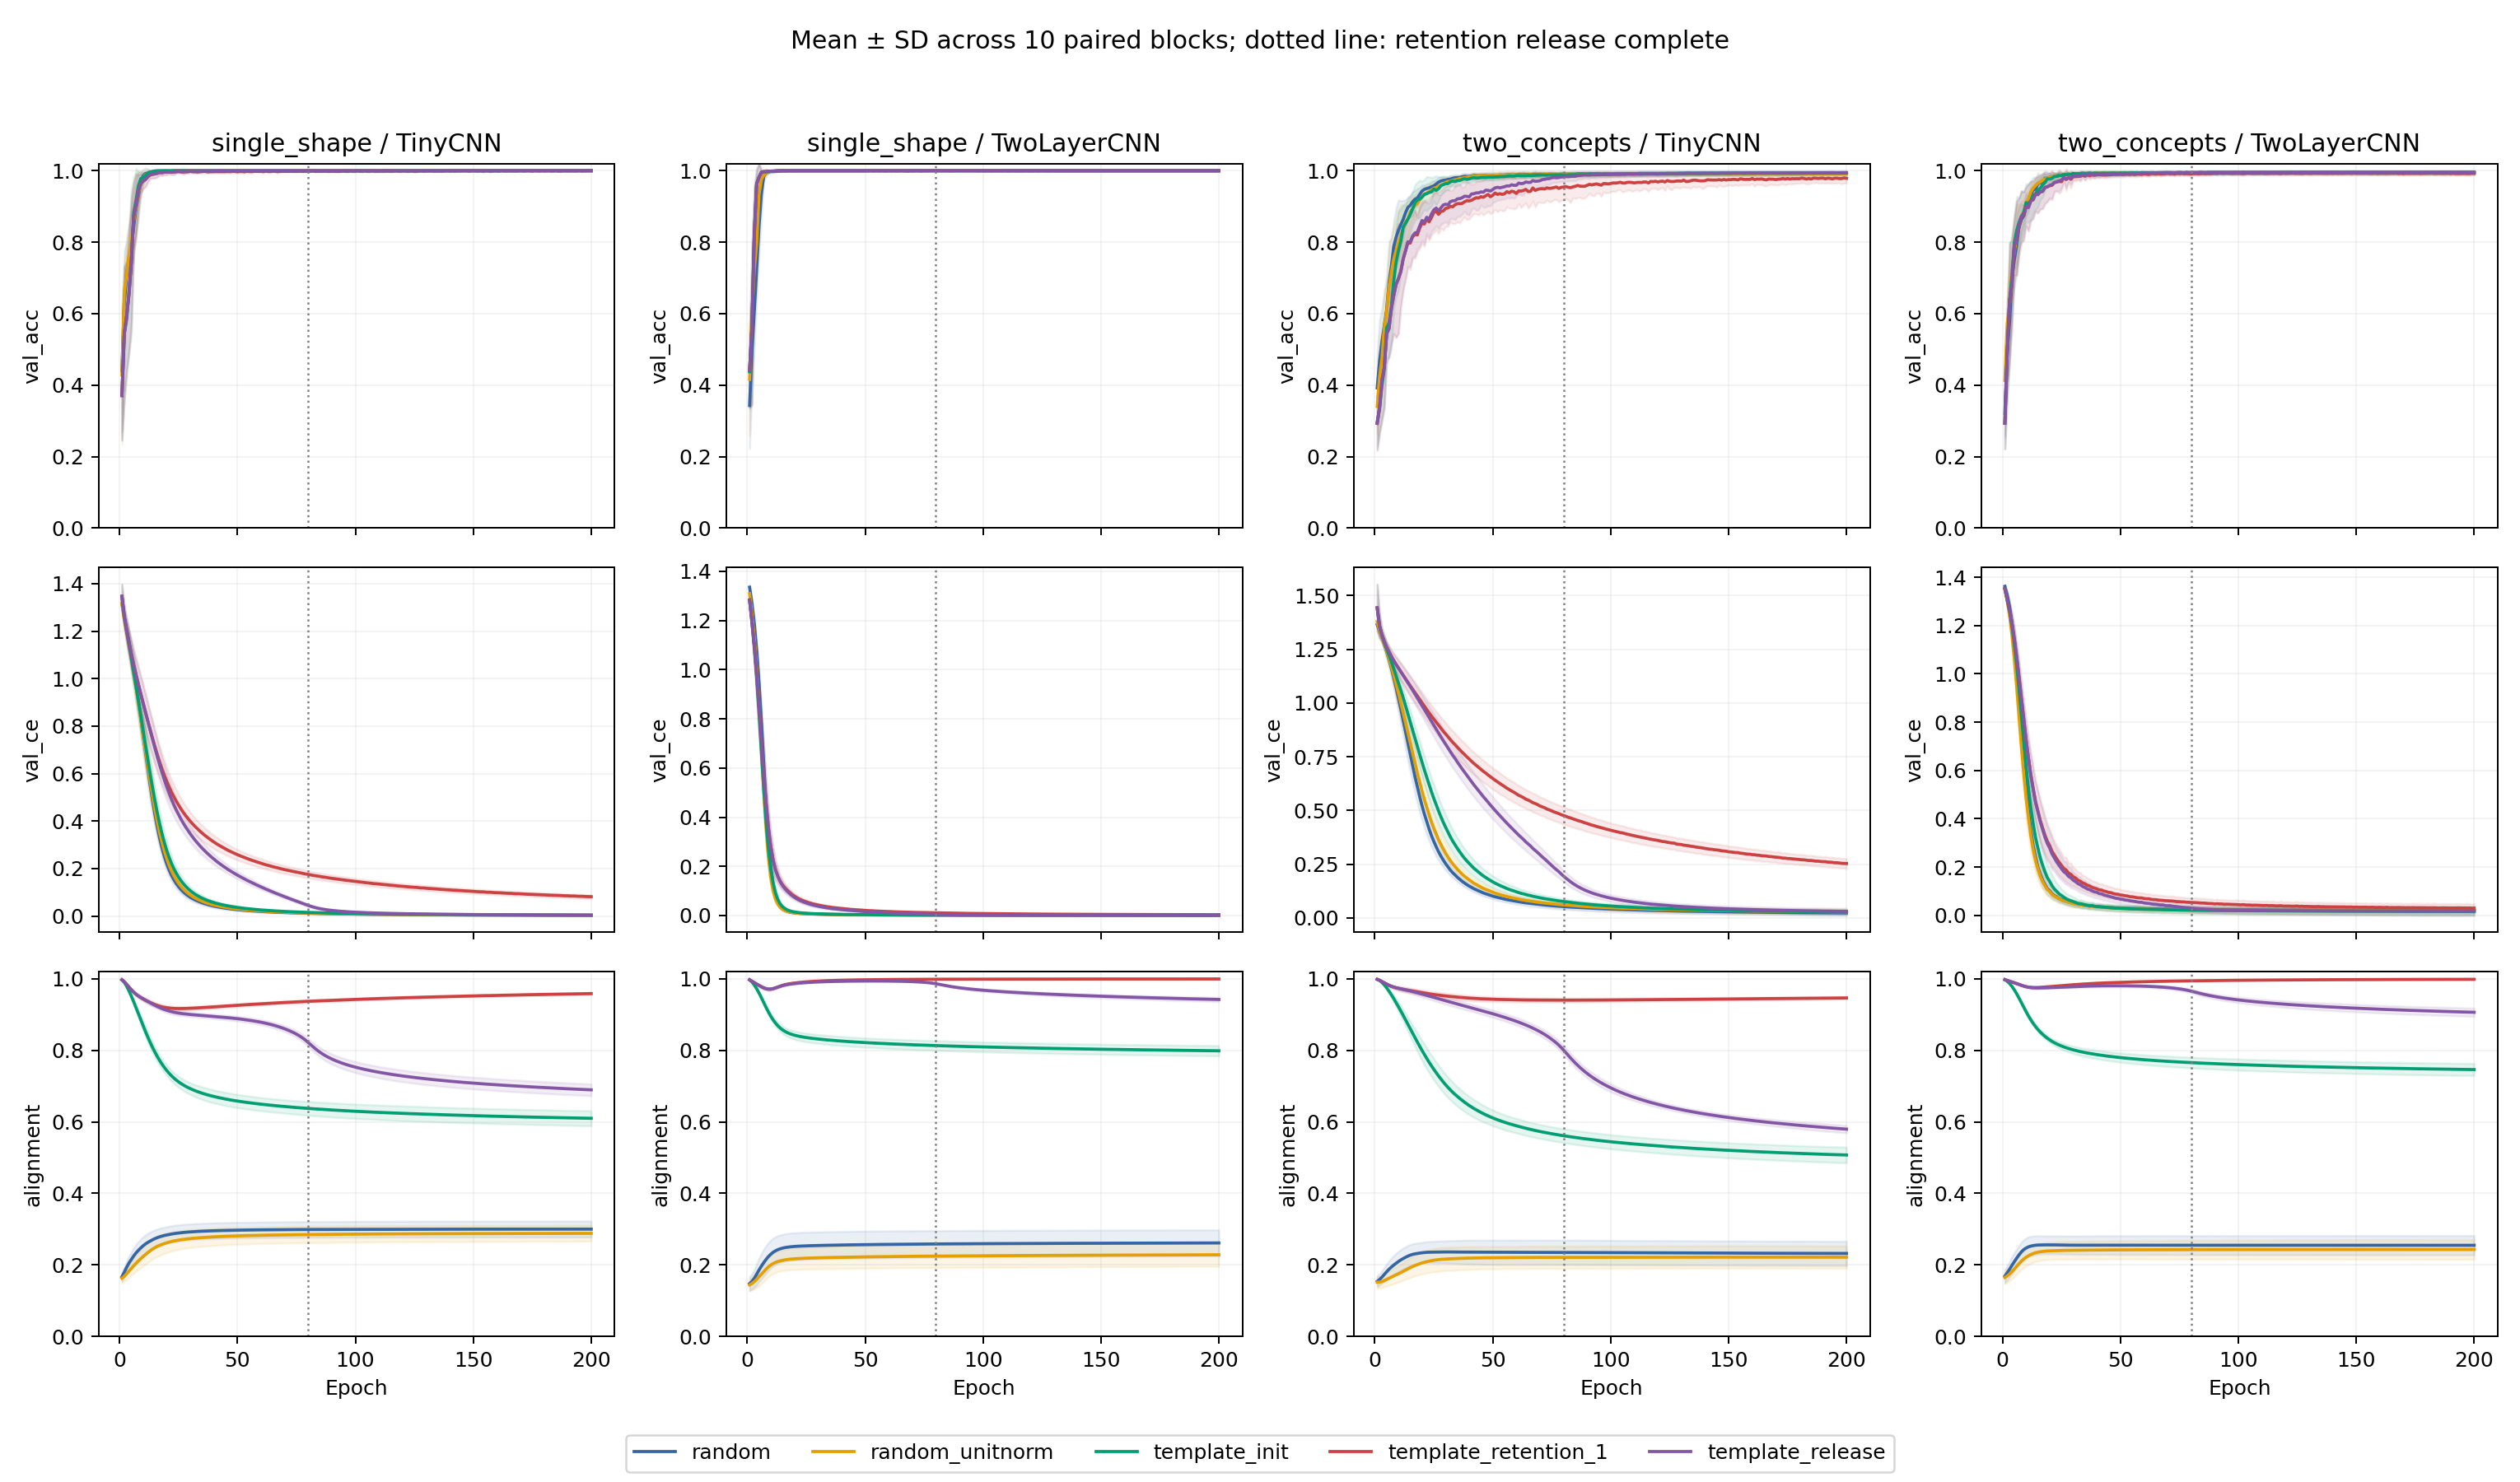
\includegraphics[width=\linewidth]{../analysis/retention_release_001/learning.png}}
\caption{Stage-B learning and alignment trajectories over 200 epochs. Curves show block means and bands show block standard deviations. Persistent retention and release separate only after the release schedule begins.}
\label{fig:learning}
\end{figure}

These results establish a tradeoff in the tested schedule: retaining the anchor strongly preserves morphology, whereas relaxing it permits lower-alignment solutions with slightly better compositional accuracy. They do not establish that reduced alignment \emph{causes} the accuracy gain.

\subsection{A fixed-budget relative score can be baseline-driven}\label{sec:decomposition}

Stage C initially appeared to show a sign reversal in \texttt{two\_concepts}/TinyCNN: release-minus-retention $U_{\mathrm{random}}$ was negative for $k=1,2$ and positive for $k=4,8$ under all three rankings. Decomposing the score changes the interpretation. Under the original contrast ranking, the exploratory release-minus-retention selected-fidelity effects were $-0.375$, $-0.163$, $-0.022$, and $+0.006$ for $k=1,2,4,8$, respectively, whereas the corresponding random-fidelity changes were $-0.040$, $-0.062$, $-0.083$, and $-0.033$. The positive $\Delta U(4)=+0.061$ therefore occurs even though selected fidelity itself is slightly lower; it is substantially created by the more negative random baseline.

The same qualitative selected-fidelity pattern appears under AUROC and validation-patch rankings: strongly negative at small budgets, near zero/slightly negative at four, and slightly positive at eight. A validation-energy-matched baseline changes the relative score but not this direct selected-fidelity observation. Matching quality is excellent for many $k=4$ and $k=8$ settings but can be poor for singleton interventions, so the energy-matched score remains a secondary diagnostic. This decomposition motivated Stage D's use of selected fidelity, rather than $U$, as the primary outcome.

\subsection{Prospective confirmation: functional conclusions shift with intervention budget}\label{sec:confirmation}

All 80 planned Stage-D models and all 80 final-checkpoint evaluations completed. The predeclared TinyCNN/contrast intervention-budget contrast is
\[
\bar B=0.330976,\qquad
95\%\ \mathrm{CI}=[0.273680,0.388273],
\]
with $t_{19}=12.0905$ and two-sided $p=2.28\times10^{-10}$. The frozen confirmation rule is therefore satisfied.

Crucially, confirmation of $B>0$ does \emph{not} mean that release improves selected fidelity at every larger budget. The four required individual effects are shown in Table~\ref{tab:primary-curve}.

\begin{table}[t]
\centering
\small
\begin{tabular}{rcc}
\toprule
Patched channels $k$ & $\Delta F_{\mathrm{selected}}$ & 95\% CI \\
\midrule
1 & $-0.3459$ & $[-0.4033,-0.2885]$ \\
2 & $-0.3317$ & $[-0.4082,-0.2552]$ \\
4 & $-0.0221$ & $[-0.0424,-0.0019]$ \\
8 & $+0.0065$ & $[+0.0037,+0.0093]$ \\
\bottomrule
\end{tabular}
\caption{Stage-D primary TinyCNN/contrast release-minus-retention selected-fidelity effects on 20 fresh \texttt{two\_concepts} blocks.}
\label{tab:primary-curve}
\end{table}

Release is therefore much less favorable for one- and two-channel interventions than for four- and eight-channel interventions; the sign becomes positive only at $k=8$. Absolute selected-patch counterfactual accuracy follows the same broad pattern: its release-minus-retention effect is $-0.2009$ at $k=1$, $-0.3626$ at $k=2$, $-0.0241$ at $k=4$, and $+0.0140$ at $k=8$.

The two alternative validation-only rankings support the same TinyCNN budget dependence as predeclared secondary analyses: $B=0.3001$ for AUROC ranking and $B=0.2305$ for validation-patch ranking, with both marginal 95\% intervals entirely positive. TwoLayerCNN differs. Its contrast-ranking $B=-0.0419$ (95\% CI $[-0.0701,-0.0137]$), AUROC $B=-0.0318$ ($[-0.0583,-0.0053]$), and validation-patch $B=+0.0116$ ($[-0.0095,0.0327]$). Thus the fresh confirmation establishes a positive budget shift in the primary shallow setting while simultaneously arguing against a universal architecture-independent direction.

The energy-matched relative score also separates small and larger budgets in TinyCNN, but it remains secondary because baseline definition changes $U$ and matching error is heterogeneous. Full-patch and no-op numerical errors were zero.

\subsection{Architecture changes the direction of the budget shift}\label{sec:exhaustive}

Stage E completed all 1,200 planned final-checkpoint evaluations on 50 fresh blocks. Under the original contrast ranking and default release schedule, the predeclared intervention-budget contrast relative to constant retention is positive for TinyCNN on both tasks and not positive for TwoLayerCNN. Table~\ref{tab:stage-e-main} puts this architecture boundary in the main paper rather than leaving it in the appendix.

\begin{table}[t]
\centering
\small
\begin{tabular}{lccc}
\toprule
Setting & Mean $B$ & 95\% CI & Holm $p$ \\
\midrule
\texttt{single\_shape} / TinyCNN & +0.07189 & [0.05444, 0.08934] & $1.43\times10^{-10}$ \\
\texttt{single\_shape} / TwoLayerCNN & -0.01018 & [-0.02290, 0.00254] & 0.4569 \\
\texttt{two\_concepts} / TinyCNN & +0.28619 & [0.25389, 0.31850] & $1.95\times10^{-22}$ \\
\texttt{two\_concepts} / TwoLayerCNN & -0.04156 & [-0.06983, -0.01329] & 0.0144 \\
\bottomrule
\end{tabular}
\caption{Stage-E default-release intervention-budget contrast relative to constant retention under the original contrast ranking. These are predeclared secondary robustness results, not additional primary tests.}
\label{tab:stage-e-main}
\end{table}

The robustness map is not specific to the default schedule. Relative to $\lambda=1$ retention, all five alternative prior profiles have positive contrast-ranking $B$ in TinyCNN for both tasks. For \texttt{two\_concepts}/TinyCNN, the values range from $0.1663$ for constant $\lambda=0.1$ to $0.3456$ for immediate release after template initialization. By contrast, TwoLayerCNN effects are near zero on \texttt{single\_shape} and tend to be negative for released profiles on \texttt{two\_concepts}. Because release timing changes several aspects of optimization jointly, these ordered schedules are interpreted as sensitivity analysis rather than a monotone causal dose law.

\begin{figure}[t]
\centering
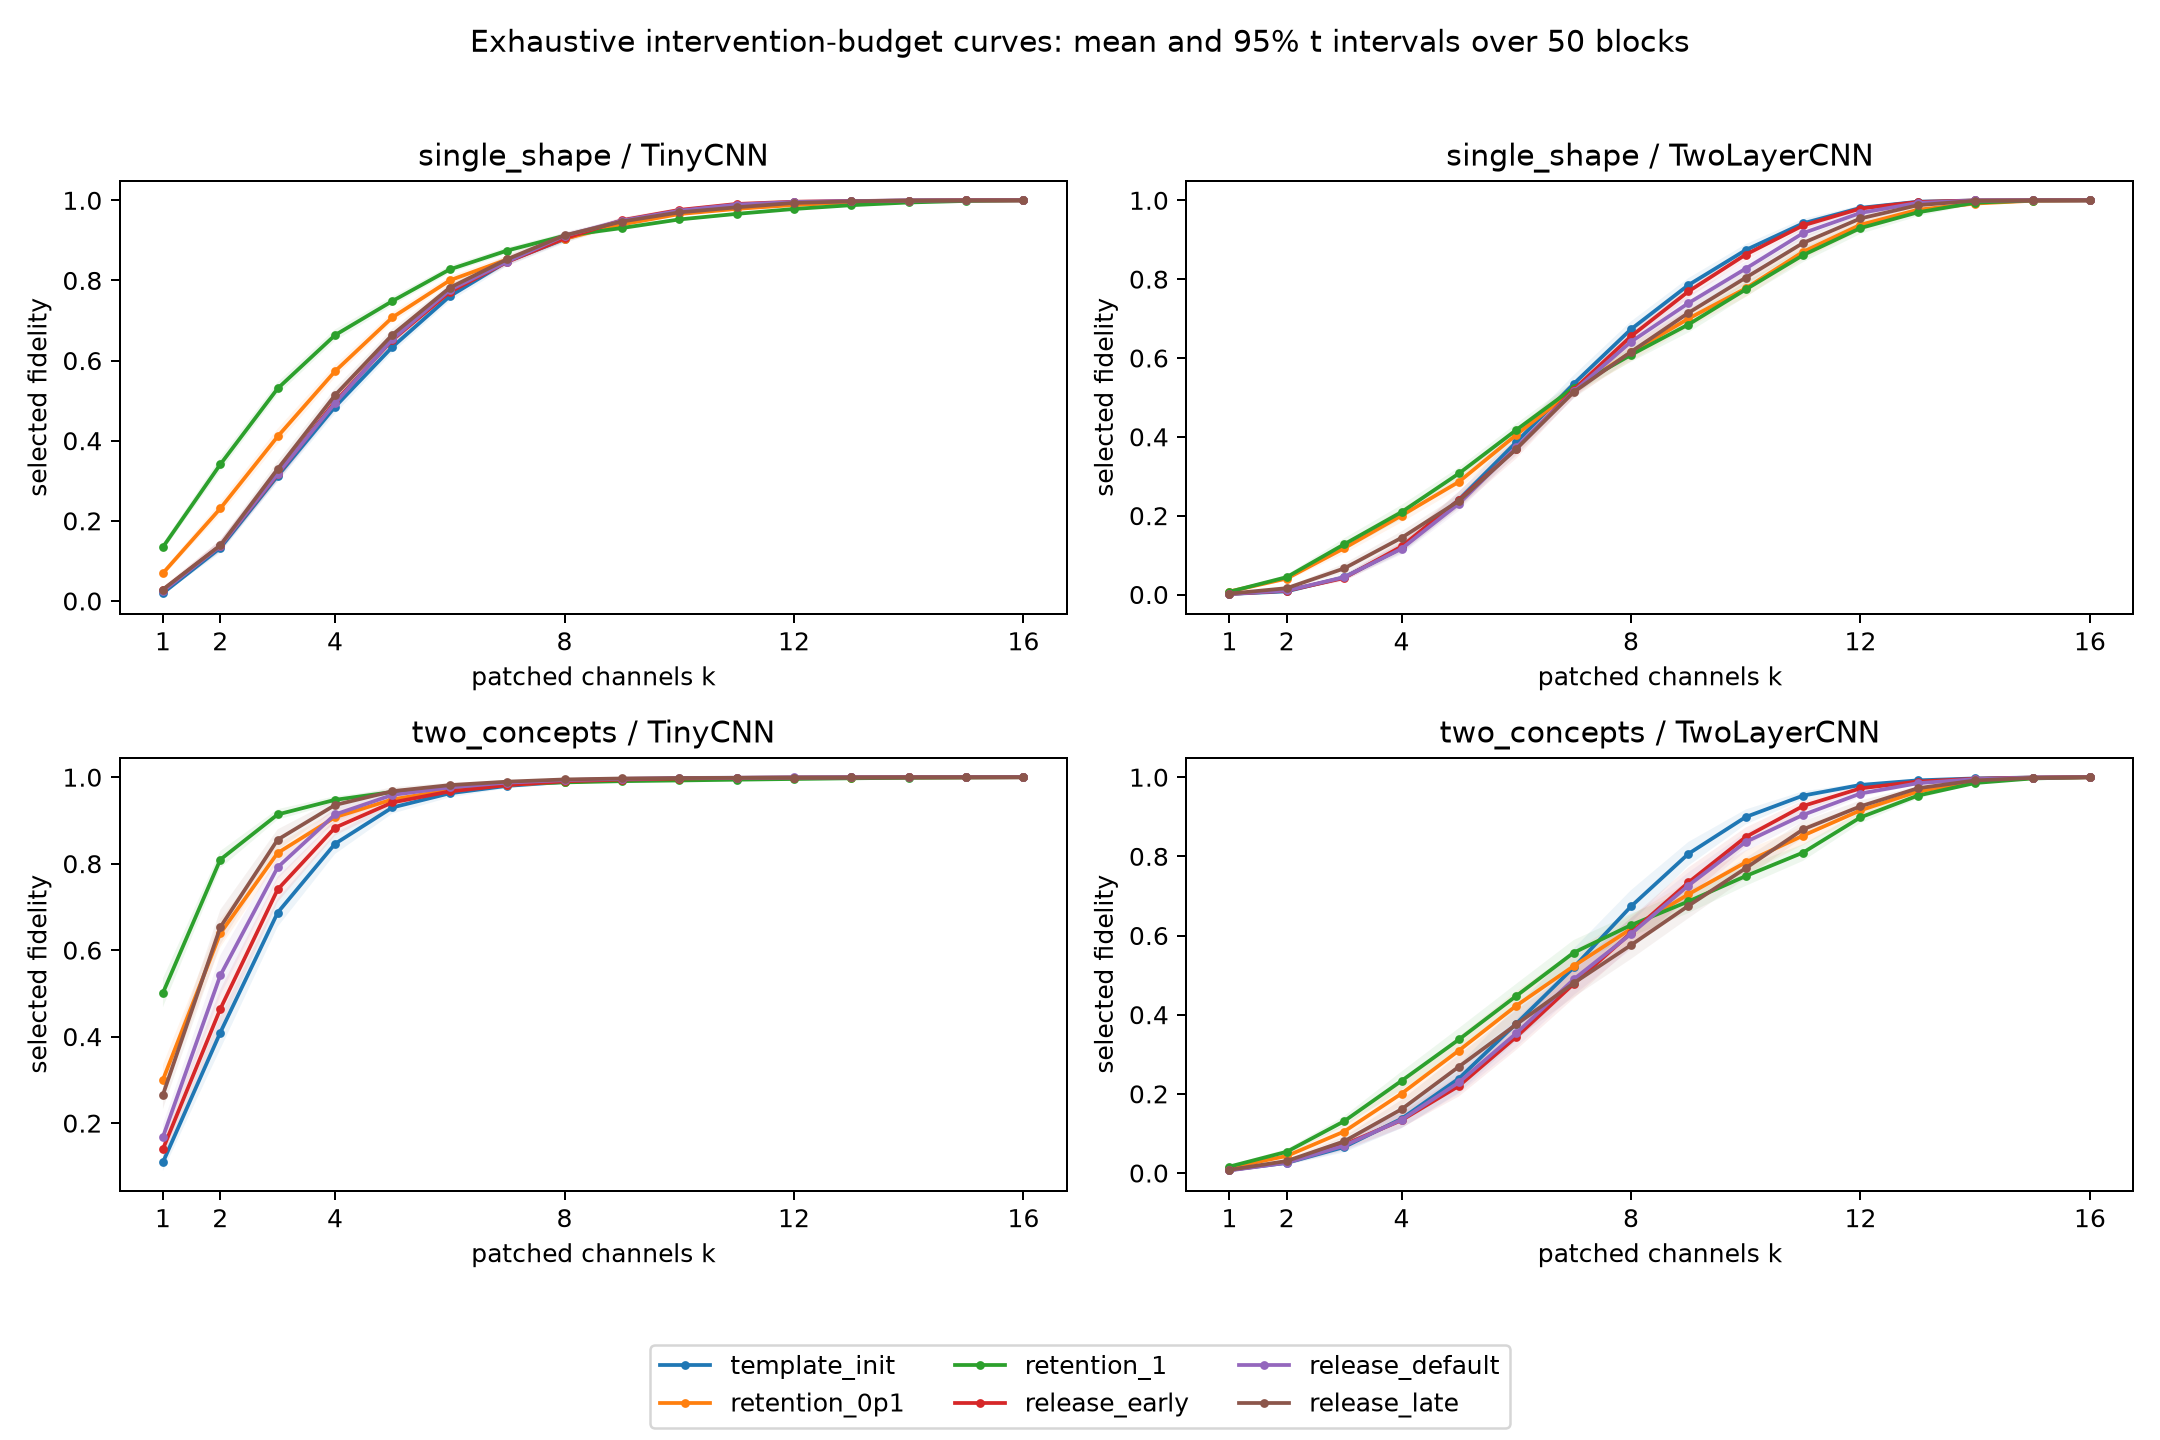
\includegraphics[width=\linewidth]{../analysis/exhaustive_robustness_001/selected_fidelity_budget_curves.png}
\caption{Stage-E selected-fidelity curves for $k=1,\ldots,16$ under the contrast ranking. Each panel contains all six template-prior profiles; lines are means over 50 fresh blocks and bands are 95\% $t$ intervals. The full-patch boundary at $k=16$ is an integrity check.}
\label{fig:exhaustive-curves}
\end{figure}

Figure~\ref{fig:exhaustive-curves} is the visual robustness counterpart to the compact statistic in Table~\ref{tab:stage-e-main}. In TinyCNN, the relative ordering of released and retained profiles changes markedly as more channels are patched; in TwoLayerCNN the corresponding treatment differences do not follow the same direction. The convergence of every curve to the full-patch boundary at $k=16$ also provides a direct integrity check on the intervention implementation.

Prediction is near saturation on \texttt{single\_shape} for all profiles, so the budget differences there are not consequences of large accuracy gaps. On \texttt{two\_concepts}/TinyCNN, constant retention has mean test accuracy 98.05\% and alignment 0.944, whereas default release has 99.45\% and alignment 0.574. On TwoLayerCNN the corresponding accuracies are 99.11\% and 99.26\%, while alignment changes from 0.999 to 0.896. Thus high retained alignment remains clearly separable from both ordinary accuracy and the direction of the intervention-budget contrast.

\subsection{Morphology remains aligned under one-to-one matching}\label{sec:matching-results}

The exploratory matching analysis on the 2,000 saved Stage-B checkpoint states asks whether the high retained-alignment result could be produced by many learned kernels repeatedly selecting the same nearest template. Maximum-weight one-to-one assignment removes that possibility by allowing each template to be used at most once. At epoch 200, one-to-one assignment similarity for constant retention ranges from 0.9468 to 0.9999 across the four task/architecture settings, with essentially zero nearest-versus-assignment gap, while release means range from 0.5743 to 0.9425. Thus the morphology contrast survives a stricter matching rule.

\begin{figure}[t]
\centering
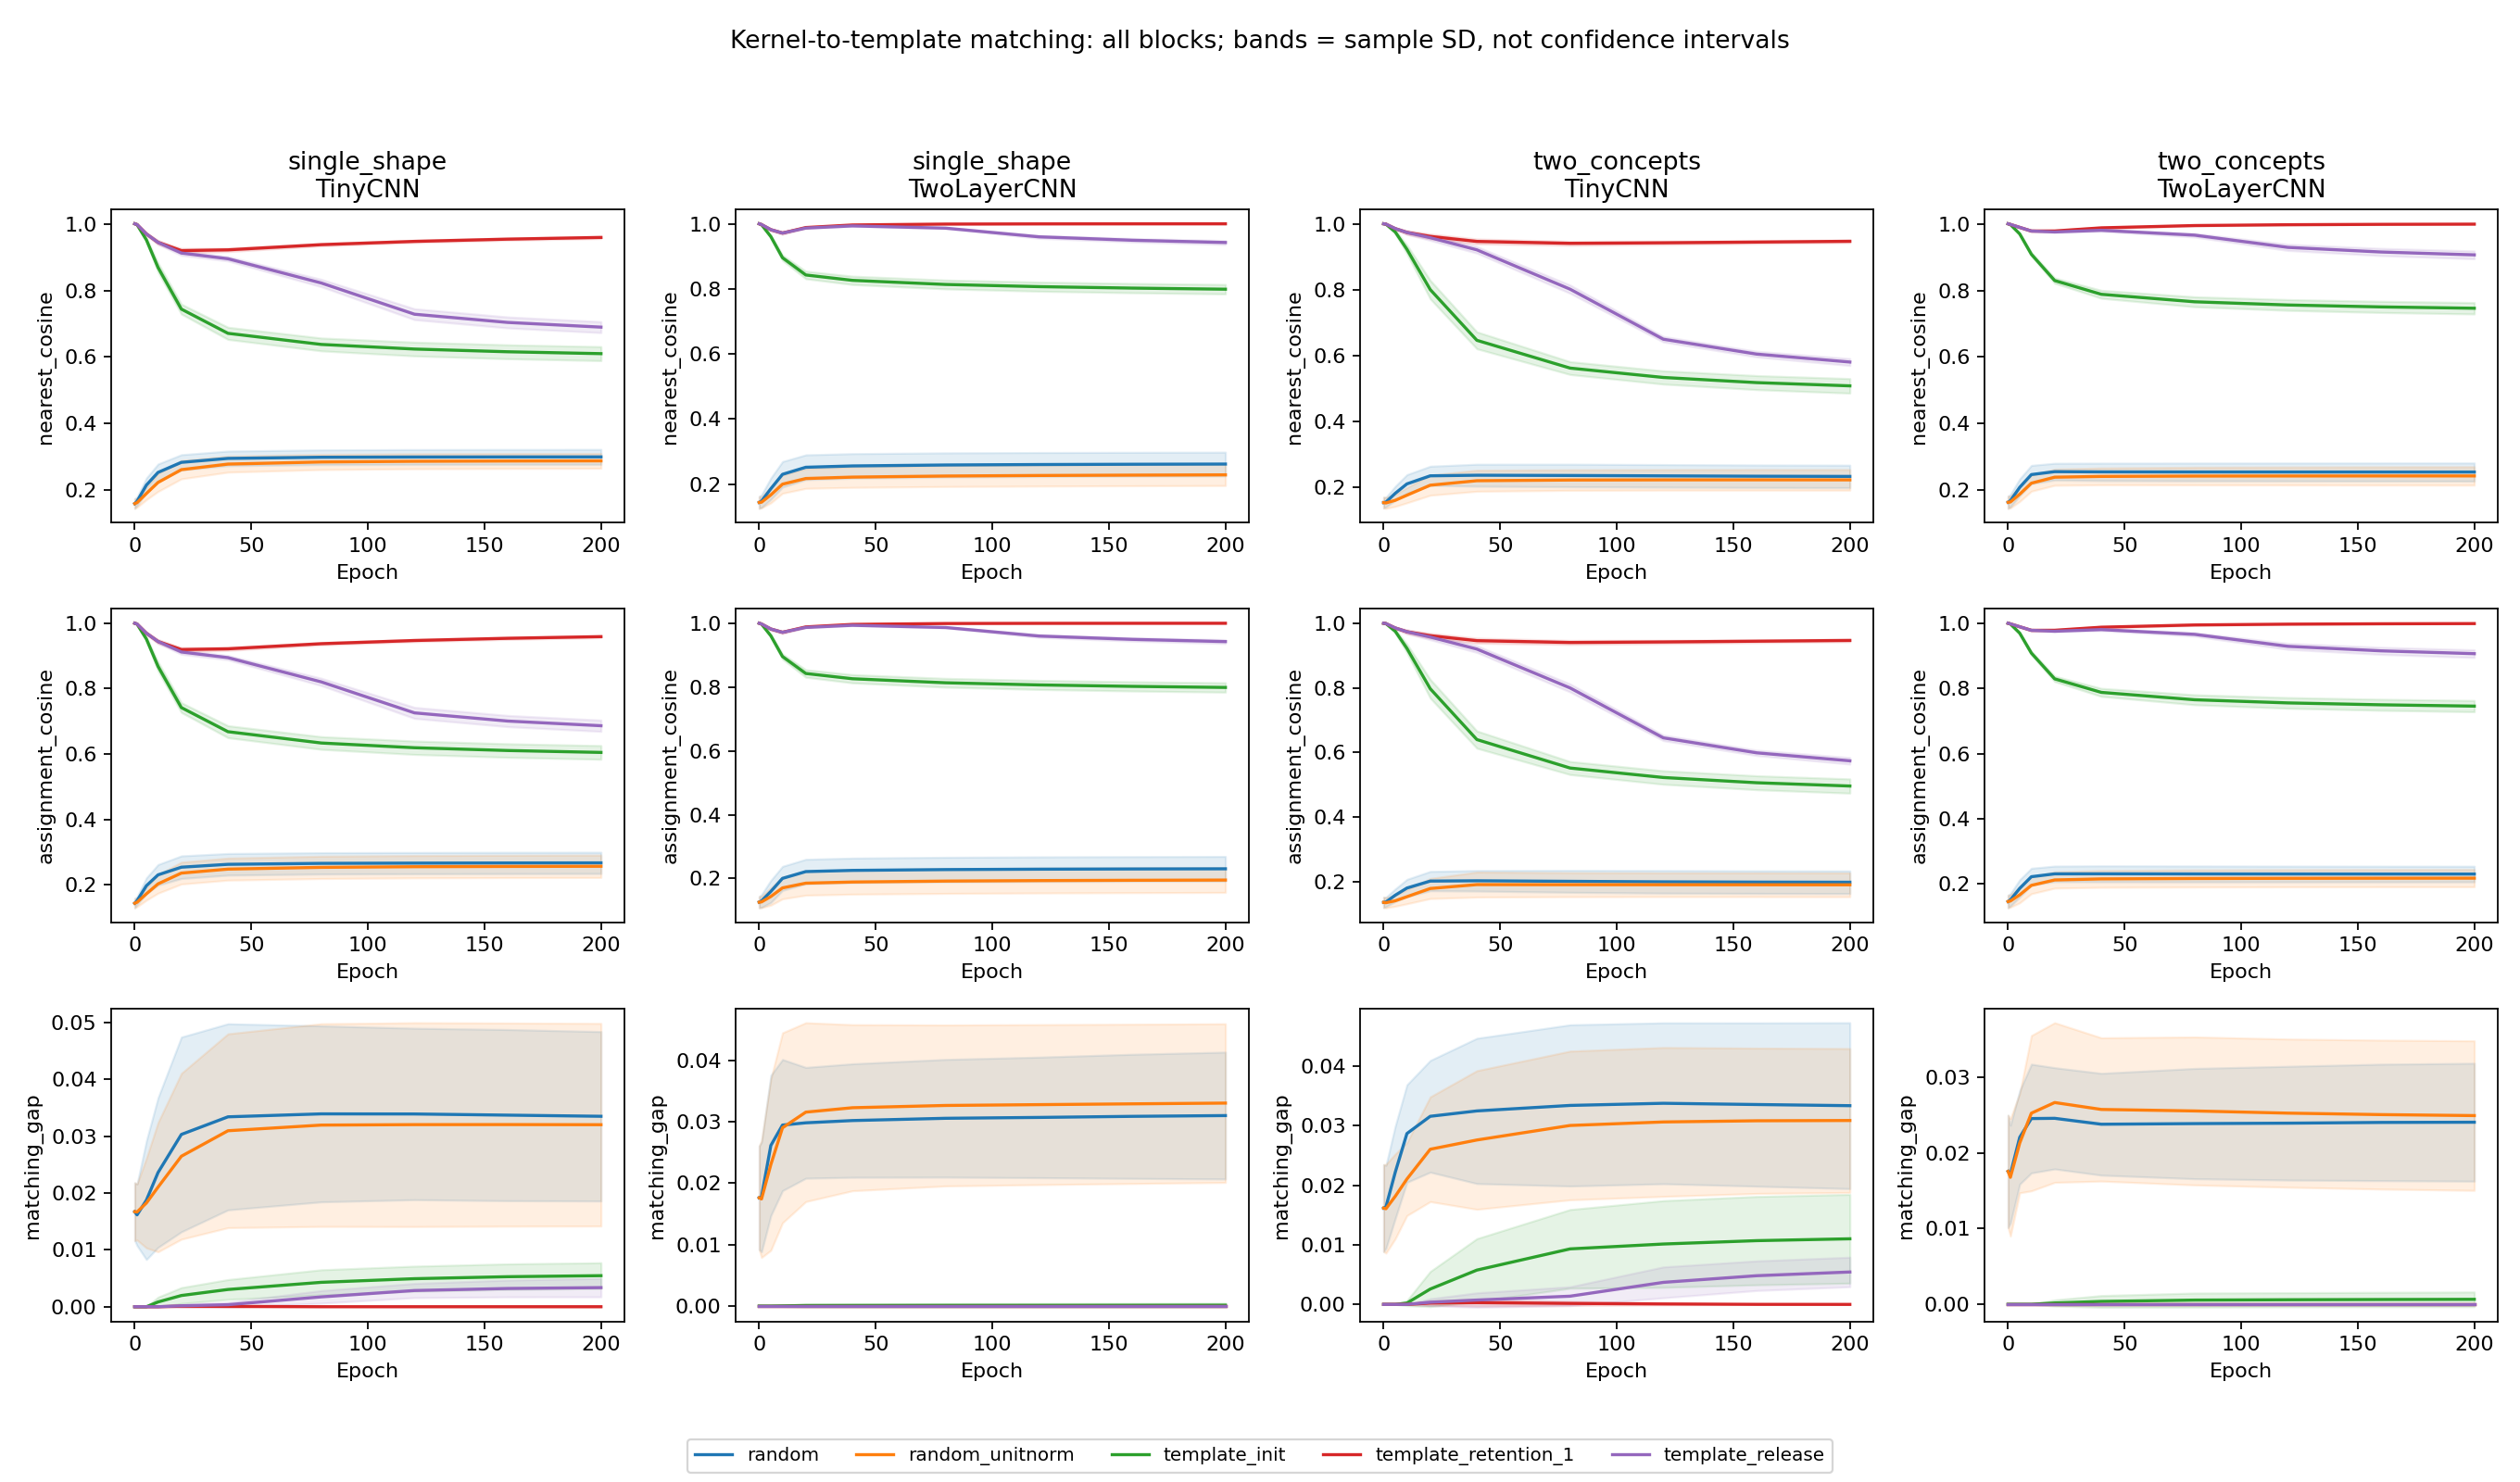
\includegraphics[width=\linewidth]{../analysis/kernel_similarity/results/matching_trajectories.png}
\caption{Nearest-template alignment, maximum-weight one-to-one alignment, and their gap over all saved Stage-B epochs. All five conditions and four task/architecture settings are shown. Bands are sample SD over ten blocks, not confidence intervals.}
\label{fig:matching-trajectories}
\end{figure}

Figure~\ref{fig:matching-trajectories} shows when this distinction emerges during learning rather than only at the endpoint. The nearest-template curve allows template reuse; the one-to-one curve does not. Their small endpoint gap under persistent retention means the high alignment is supported by distinct channel--template assignments rather than by a few templates being reused across many channels. Release follows a lower-alignment trajectory after the constraint is relaxed, consistent with the weight-space tradeoff already seen in Figure~\ref{fig:learning}.

\begin{figure}[t]
\centering
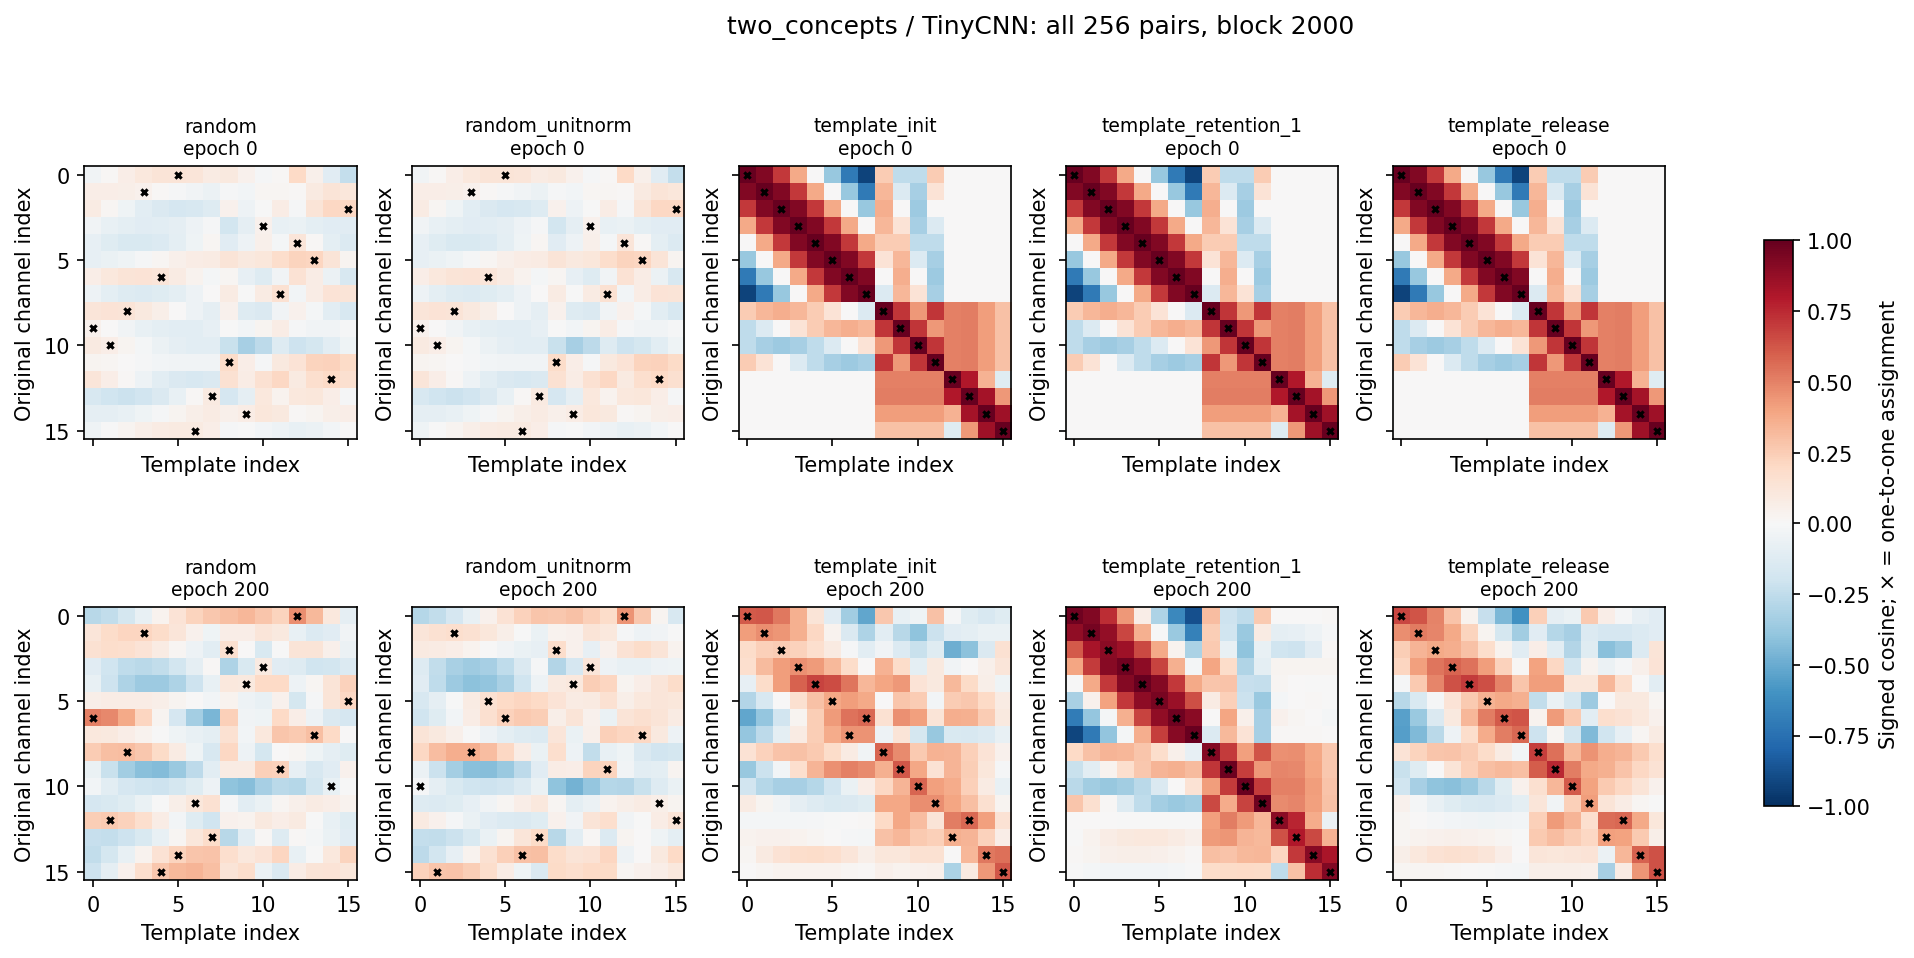
\includegraphics[width=\linewidth]{../analysis/kernel_similarity/results/matrices_two_concepts_TinyCNN.png}
\caption{All 256 signed kernel--template cosine similarities for \texttt{two\_concepts}/TinyCNN, fixed block 2000, at initialization and epoch 200. Rows retain original channel indices and columns retain template indices; black crosses mark the maximum-weight one-to-one assignment. Values range from $-1$ to $1$.}
\label{fig:matching-matrices}
\end{figure}

Figure~\ref{fig:matching-matrices} opens the aggregate alignment score into the full $16\times16$ channel--template similarity structure for a fixed block. Each black cross is one pairing used by the assignment score, so the reader can see exactly which matrix entries contribute to the one-to-one summary and how those pairings change between initialization and epoch 200. This is useful as an audit of the aggregate morphology statistic: the figure displays the complete similarity information rather than only the maximum selected for each channel.

\begin{figure}[t]
\centering
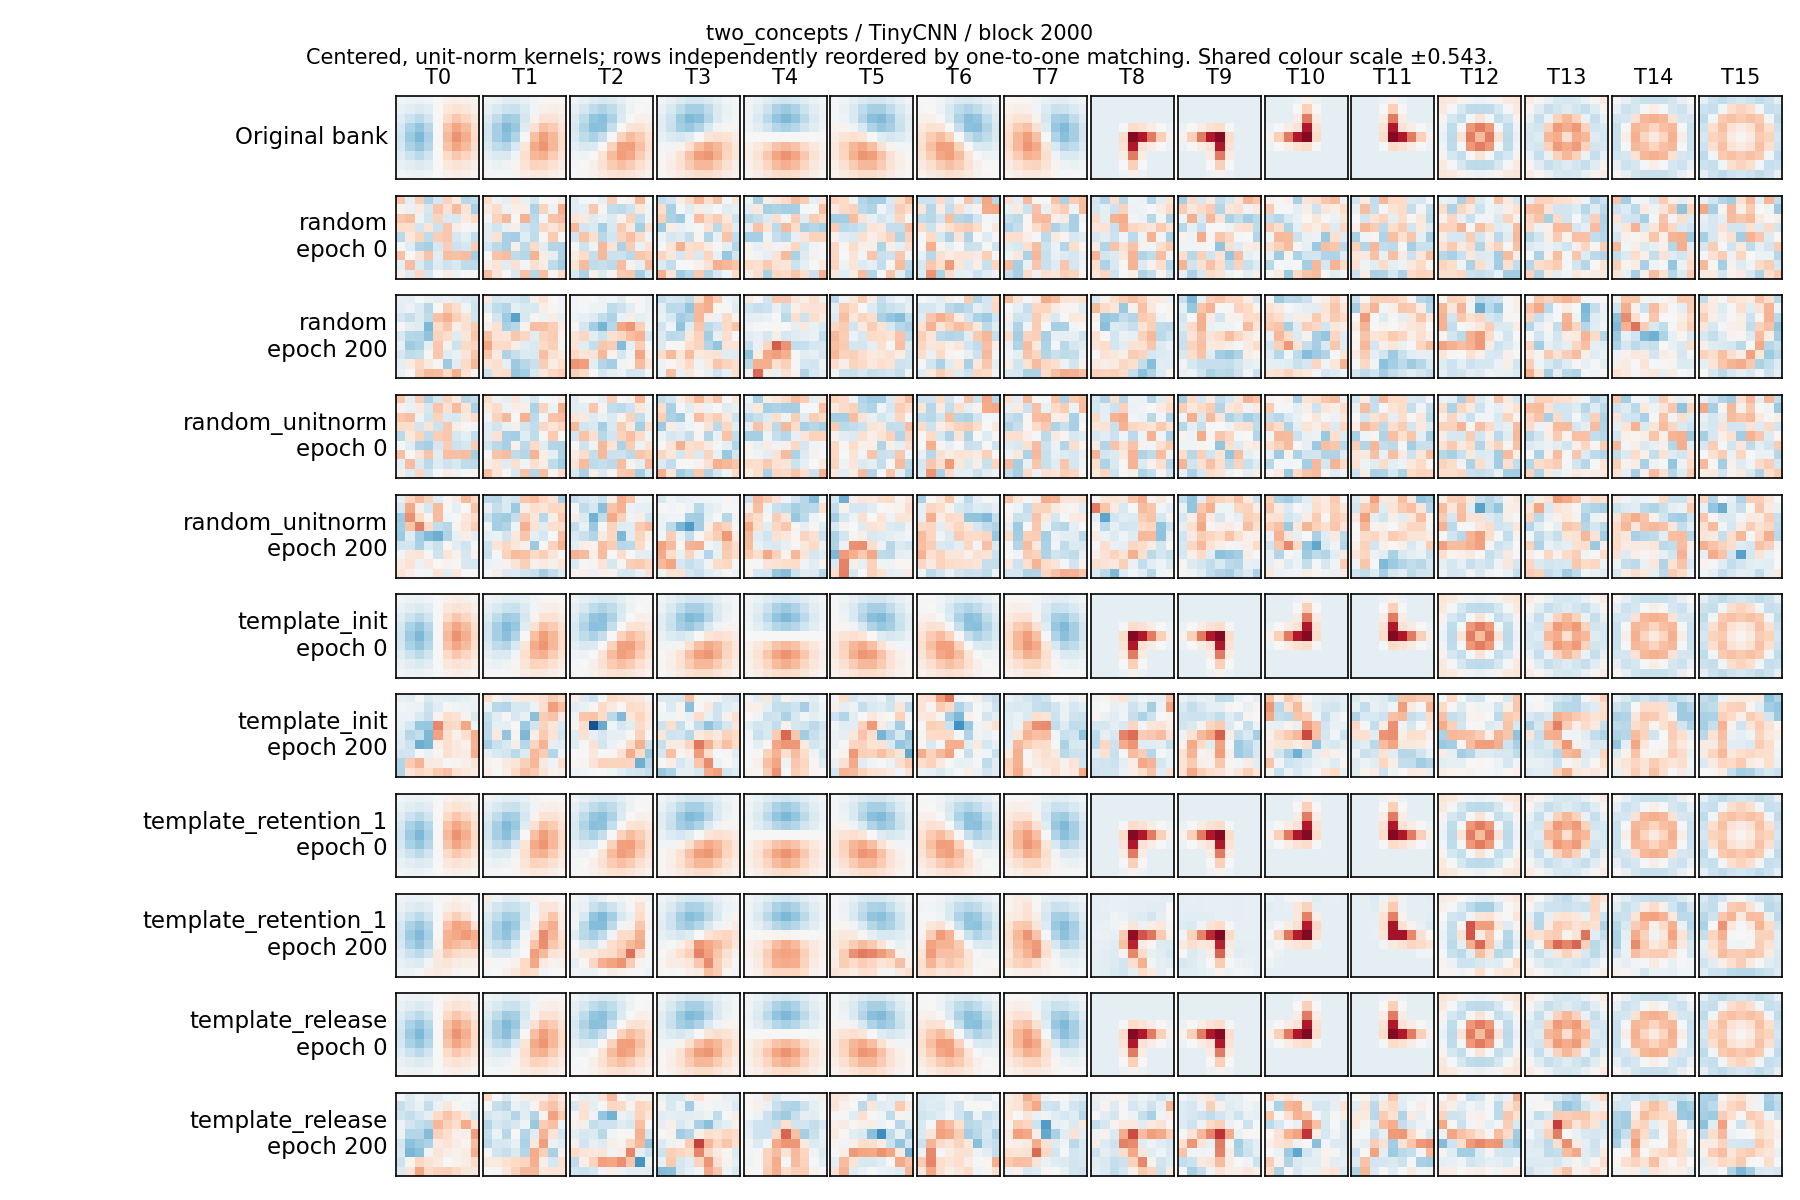
\includegraphics[width=\linewidth]{../analysis/kernel_similarity/results/kernels_two_concepts_TinyCNN.png}
\caption{Original templates and saved first-layer kernels for \texttt{two\_concepts}/TinyCNN, block 2000. Rows are independently reordered by maximum-weight one-to-one matching so that the paired template and learned kernel can be compared directly. The illustration concerns morphology, not human interpretability.}
\label{fig:kernel-gallery}
\end{figure}

The gallery in Figure~\ref{fig:kernel-gallery} complements the trajectory and matrix views by showing the filters themselves after assignment. Together, Figures~\ref{fig:matching-trajectories}--\ref{fig:kernel-gallery} support only a morphology statement: persistent retention preserves a bank of kernels that remains close to distinct predefined templates, whereas release permits larger drift. They do not establish semantic uniqueness, human readability, or the mechanism behind the patching curves. The complete endpoint matching table is retained in Appendix~\ref{app:kernel-matching}.

\section{Interpretation}\label{sec:interpretation}

The headline is not that template priors fail, nor that release ``wins.'' It is that template appearance and intervention-based function are distinct empirical objects. Persistent retention yields near-template morphology, yet the release-minus-retention intervention effect changes dramatically with patch budget and can change direction with architecture. A single fixed-budget score can therefore give an incomplete---and in some settings qualitatively different---answer about the same trained models.

Three conclusions support that framing. First, template initialization and persistent template retention are different interventions. Initialization can help, hurt, or become irrelevant depending on task and architecture, while constant retention predictably preserves morphology and can impose a residual optimization cost. Second, weight-space alignment, concept discrimination, localization, selected intervention fidelity, and selected-versus-control usefulness are not interchangeable. The original $U$ analysis makes this concrete: changing the baseline can create a positive relative difference even when selected fidelity does not improve. Third, the release-versus-retention comparison in selected fidelity is genuinely budget-sensitive in the shallow compositional setting. This last statement is no longer merely post hoc: it was frozen as a single primary test and confirmed on new blocks.

What the experiments do \emph{not} establish is equally important. A positive $B$ does not show that release redistributes ``causal information'' across channels. The same observed curve could arise from redundancy, nonlinear channel interactions, ranking behavior, changes in activation scale, or the fact that patched activation combinations depart from naturally co-occurring internal states. Stage E shows that added depth changes the direction of $B$, further arguing against a single mechanism inferred from TinyCNN alone.

The most defensible interpretation is therefore measurement-level: the estimated effect of a template-retention schedule on internal intervention fidelity depends strongly on how many channels are intervened on, and that dependence itself is architecture-sensitive. This conclusion is narrower than a mechanistic explanation but stronger than the earlier exploratory observation because it is supported by fresh prospective data and a separate large robustness sample.

\section{Limitations}\label{sec:limitations}

\begin{itemize}
\item Only two related synthetic tasks, two small architectures, one first-layer template bank, and one family of optimizers/schedules are studied. There is no natural-image benchmark or human-readability experiment.
\item The renderer provides balanced, matched counterfactuals and exact object masks. This control is useful for measurement but simplifies correlations and nuisance structure found in real data.
\item The confirmed Stage-D claim is specific to \texttt{two\_concepts}/TinyCNN, the contrast ranking, epoch 200, and budgets $\{1,2,4,8\}$. Stage-E evidence broadens robustness but remains secondary.
\item Stage E explores six prior profiles and all $k=1,\ldots,16$. Holm adjustment is applied only within the predeclared five-profile families; the study is not a license to select arbitrary favorable subgroups.
\item Activation patching changes complete first-layer feature maps and can create internal combinations that are not on the model's natural activation manifold. Fidelity is tied to probability outputs and the chosen layer/ranking; other intervention metrics may differ \citep{zhang_2024_activation-patching,heimersheim_2024_activation-patching}.
\item $U_{\mathrm{random}}$ and $U_{\mathrm{energy}}$ are relative scores. The random baseline changes with budget, while energy matching is imperfect, especially for singleton interventions. Neither relative score should replace the directly reported selected fidelity.
\item The one-to-one matching result concerns a redundant rank-10 template bank and does not validate human interpretability or independent semantic coverage.
\item The independent audit covers 32 fixed Stage-B checkpoint evaluations rather than every checkpoint from every stage. Passing the audit supports the sampled implementation but is not external replication.
\end{itemize}

\section{Scope and future work}\label{sec:future}

The next scientific step is no longer to ask whether the shallow selected-fidelity contrast depends on budget; that question has been prospectively confirmed within this setting. The more consequential question is \emph{why}. A mechanism-focused follow-up should predeclare measurements of channel redundancy, joint versus singleton effects, subspace-level interventions, activation-scale controls, and architecture-by-budget interactions. It should also move beyond the present renderer to tasks with richer concept correlations and, where interpretability is claimed, include human evaluation rather than inferring readability from filter morphology.

Natural-image experiments would test external validity, while larger architectures could determine whether the TwoLayerCNN reversal is a depth effect, an optimization effect, or a peculiarity of the present small network. Alternative intervention targets and output metrics would further test whether the confirmed intervention-budget contrast is specific to first-layer probability-space patching.

\section{Conclusion}\label{sec:conclusion}

Template alignment is not functional alignment in these small CNNs. Persistent retention can make first-layer kernels look strikingly similar to predefined edge, corner, and ring templates, but that weight-space regularity does not determine a stable intervention advantage. In the prospectively confirmed TinyCNN setting, the direct release-versus-retention selected-fidelity effect is strongly negative at small patch budgets, approaches zero at four channels, and becomes slightly positive at eight; a separate 1,200-model robustness study reproduces the positive budget shift for TinyCNN while showing that TwoLayerCNN behaves differently. Baseline choice can also change the sign of a relative usefulness comparison. The practical lesson is therefore not simply to inspect more kernels or report one patching score: what a feature looks like and what an intervention says it does should be reported separately, and intervention budget, baseline definition, and architecture are part of the empirical claim rather than nuisance details.

\section{Data and code availability}\label{sec:availability}

The experiments use procedurally rendered synthetic images. The research artifact contains renderer, training and evaluation code, frozen protocols, execution manifests, checkpoint-level metrics, complete result tables, and analysis scripts. The Stage-D and Stage-E paper-facing outputs include all planned models and full numerical tables; the independent checkpoint audit protocol and report are also retained. The anonymous manuscript does not link the current working repository because that repository identifies the authors. An anonymized archival artifact and DOI should be prepared before final submission if required by the venue.

\bibliography{../literature/references.bib}

\clearpage
\appendix
\noindent\textbf{Appendix organization.} Appendix~\ref{app:confirmation} contains the complete fresh-data confirmation and robustness details; Appendix~\ref{app:historical} preserves the earlier exploratory stages that motivated the confirmatory estimand; Appendix~\ref{app:kernel-matching} retains the complete endpoint kernel-matching table corresponding to the morphology figures promoted to the main Results section.

\section{Prospective confirmation and exhaustive robustness details}\label{app:confirmation}

This appendix contains the complete numerical support for the fresh-data stages summarized in the main text. Stage D was frozen before any block 4000--4019 outcome was generated. Stage E was separately frozen before any block 5000--5049 outcome was generated and remains secondary to Stage D. The main paper now carries the headline Stage-D curve, the default-release Stage-E architecture comparison, and the full budget-curve figure; this appendix retains the complete ranking/profile breakdowns, secondary controls, and audit details. Machine-readable tables are retained under \texttt{analysis/budget\_confirmation\_001/} and \texttt{analysis/exhaustive\_robustness\_001/}.

\subsection{Stage-D selected-fidelity treatment effects}\label{app:stage-d-full}

All entries are release minus constant-retention selected fidelity at epoch 200, paired over 20 fresh blocks. Only TinyCNN/contrast supplies the single primary test; the remaining rows are predeclared secondary analyses.

{
\small
\setlength{\tabcolsep}{4pt}
\begin{longtable}{llrcc}
\caption{Stage-D release-minus-retention selected-fidelity effects.}\label{tab:stage-d-full}\\
\toprule
Architecture & Ranking & $k$ & Mean $\Delta F$ & 95\% $t$ interval \\
\midrule
\endfirsthead
\toprule
Architecture & Ranking & $k$ & Mean $\Delta F$ & 95\% $t$ interval \\
\midrule
\endhead
\bottomrule
\endfoot
TinyCNN & contrast & 1 & -0.3459 & [-0.4033, -0.2885] \\
TinyCNN & contrast & 2 & -0.3317 & [-0.4082, -0.2552] \\
TinyCNN & contrast & 4 & -0.0221 & [-0.0424, -0.0019] \\
TinyCNN & contrast & 8 & +0.0065 & [+0.0037, +0.0093] \\
TinyCNN & AUROC & 1 & -0.3040 & [-0.3662, -0.2418] \\
TinyCNN & AUROC & 2 & -0.3237 & [-0.3988, -0.2485] \\
TinyCNN & AUROC & 4 & -0.0332 & [-0.0696, +0.0032] \\
TinyCNN & AUROC & 8 & +0.0058 & [+0.0026, +0.0091] \\
TinyCNN & validation patch & 1 & -0.2856 & [-0.3191, -0.2520] \\
TinyCNN & validation patch & 2 & -0.1733 & [-0.2068, -0.1399] \\
TinyCNN & validation patch & 4 & -0.0052 & [-0.0202, +0.0098] \\
TinyCNN & validation patch & 8 & +0.0073 & [+0.0047, +0.0098] \\
TwoLayerCNN & contrast & 1 & -0.0117 & [-0.0202, -0.0032] \\
TwoLayerCNN & contrast & 2 & -0.0378 & [-0.0493, -0.0263] \\
TwoLayerCNN & contrast & 4 & -0.1313 & [-0.1645, -0.0980] \\
TwoLayerCNN & contrast & 8 & -0.0020 & [-0.0493, +0.0453] \\
TwoLayerCNN & AUROC & 1 & -0.0141 & [-0.0224, -0.0058] \\
TwoLayerCNN & AUROC & 2 & -0.0438 & [-0.0565, -0.0311] \\
TwoLayerCNN & AUROC & 4 & -0.1319 & [-0.1614, -0.1025] \\
TwoLayerCNN & AUROC & 8 & +0.0104 & [-0.0402, +0.0611] \\
TwoLayerCNN & validation patch & 1 & -0.0256 & [-0.0380, -0.0131] \\
TwoLayerCNN & validation patch & 2 & -0.0760 & [-0.1048, -0.0473] \\
TwoLayerCNN & validation patch & 4 & -0.0883 & [-0.1401, -0.0365] \\
TwoLayerCNN & validation patch & 8 & +0.0100 & [-0.0015, +0.0214] \\
\end{longtable}
\normalsize
}

\subsection{Stage-D intervention-budget contrasts}\label{app:stage-d-b}

For every architecture/ranking pair, the intervention-budget contrast is
\[
B=\frac{\Delta F(4)+\Delta F(8)}{2}-\frac{\Delta F(1)+\Delta F(2)}{2}.
\]
Positive $B$ means release becomes relatively more faithful at the larger tested intervention budgets; it does not require a positive release effect at each larger $k$. The TinyCNN/contrast row is the single frozen primary test. All other rows are secondary and do not alter the primary decision.

\begin{table}[h]
\centering
\small
\begin{tabular}{llccc}
\toprule
Architecture & Ranking & Mean $B$ & 95\% CI & two-sided $p$ \\
\midrule
TinyCNN & contrast & +0.33098 & [0.27368, 0.38827] & $2.28\times10^{-10}$ \\
TinyCNN & AUROC & +0.30014 & [0.24866, 0.35162] & $1.95\times10^{-10}$ \\
TinyCNN & validation patch & +0.23050 & [0.20442, 0.25658] & $1.31\times10^{-13}$ \\
TwoLayerCNN & contrast & -0.04189 & [-0.07010, -0.01367] & 0.00580 \\
TwoLayerCNN & AUROC & -0.03179 & [-0.05830, -0.00529] & 0.02126 \\
TwoLayerCNN & validation patch & +0.01162 & [-0.00949, 0.03273] & 0.26368 \\
\bottomrule
\end{tabular}
\caption{Stage-D intervention-budget contrasts. The first row alone is confirmatory.}
\label{tab:stage-d-b}
\end{table}

\subsection{Stage-D absolute counterfactual accuracy}\label{app:stage-d-cf}

Absolute selected-patch counterfactual accuracy was retained to prevent a relative fidelity score from obscuring the direction of intervention correctness. For the primary TinyCNN/contrast setting, release minus retention is $-0.2009$ at $k=1$, $-0.3626$ at $k=2$, $-0.0241$ at $k=4$, and $+0.0140$ at $k=8$. The corresponding 95\% intervals are $[-0.2551,-0.1466]$, $[-0.4400,-0.2852]$, $[-0.0524,0.0042]$, and $[0.0086,0.0193]$.

The same qualitative small-versus-larger-budget separation appears under AUROC and validation-patch rankings. These are secondary outcomes and were not used to define confirmation.

\subsection{Energy-matched control}\label{app:energy-control}

The validation-energy-matched control selects eight same-size alternative channel sets with replacement energy closest to the selected set, using validation data only. For TinyCNN/contrast, release-minus-retention $U_{\mathrm{energy}}$ is -0.2980 at $k=1$, -0.1887 at $k=2$, +0.1310 at $k=4$, and +0.0696 at $k=8$. Matching quality is not uniform: singleton alternatives can be poorly matched, whereas $k=4$ and $k=8$ are generally much tighter. The control therefore supports sensitivity of relative scores to intervention size but is not substituted for selected fidelity in the primary analysis.

\subsection{Stage-E full profile map under contrast ranking}\label{app:stage-e-profiles}

The four default-release rows that delimit the architecture effect are promoted to Table~\ref{tab:stage-e-main} in the main paper. The table below gives the complete five-profile-versus-retention family for each task/architecture setting. Holm adjustment is performed within each task/architecture/ranking family, exactly as predeclared.

{
\small
\setlength{\tabcolsep}{3.5pt}
\begin{longtable}{lllccl}
\caption{Stage-E intervention-budget contrasts for every non-reference profile under contrast ranking.}\label{tab:stage-e-profiles}\\
\toprule
Task & Architecture & Profile vs. retention 1 & Mean $B$ & 95\% CI & Holm $p$ \\
\midrule
\endfirsthead
\toprule
Task & Architecture & Profile vs. retention 1 & Mean $B$ & 95\% CI & Holm $p$ \\
\midrule
\endhead
\bottomrule
\endfoot
single shape & TinyCNN & template init & +0.06804 & [0.05343, 0.08264] & $6.91\times10^{-12}$ \\
single shape & TinyCNN & retention 0.1 & +0.03871 & [0.02525, 0.05218] & $5.13\times10^{-7}$ \\
single shape & TinyCNN & release early & +0.06855 & [0.05228, 0.08482] & $1.11\times10^{-10}$ \\
single shape & TinyCNN & release default & +0.07189 & [0.05444, 0.08934] & $1.43\times10^{-10}$ \\
single shape & TinyCNN & release late & +0.07955 & [0.06404, 0.09505] & $3.61\times10^{-13}$ \\
single shape & TwoLayerCNN & template init & +0.00762 & [-0.00793, 0.02317] & 0.9885 \\
single shape & TwoLayerCNN & retention 0.1 & +0.00031 & [-0.01053, 0.01116] & 1.0000 \\
single shape & TwoLayerCNN & release early & +0.00003 & [-0.01500, 0.01506] & 1.0000 \\
single shape & TwoLayerCNN & release default & -0.01018 & [-0.02290, 0.00254] & 0.4569 \\
single shape & TwoLayerCNN & release late & -0.01237 & [-0.02194, -0.00279] & 0.0621 \\
two concepts & TinyCNN & template init & +0.34557 & [0.31797, 0.37317] & $5.61\times10^{-29}$ \\
two concepts & TinyCNN & retention 0.1 & +0.16626 & [0.14002, 0.19251] & $3.71\times10^{-17}$ \\
two concepts & TinyCNN & release early & +0.32245 & [0.28415, 0.36074] & $1.26\times10^{-21}$ \\
two concepts & TinyCNN & release default & +0.28619 & [0.25389, 0.31850] & $1.95\times10^{-22}$ \\
two concepts & TinyCNN & release late & +0.19342 & [0.16432, 0.22253] & $1.20\times10^{-17}$ \\
two concepts & TwoLayerCNN & template init & -0.00583 & [-0.03214, 0.02049] & 0.6583 \\
two concepts & TwoLayerCNN & retention 0.1 & -0.01413 & [-0.03880, 0.01054] & 0.5104 \\
two concepts & TwoLayerCNN & release early & -0.04199 & [-0.06889, -0.01509] & 0.0116 \\
two concepts & TwoLayerCNN & release default & -0.04156 & [-0.06983, -0.01329] & 0.0144 \\
two concepts & TwoLayerCNN & release late & -0.04523 & [-0.06854, -0.02192] & 0.00147 \\
\end{longtable}
\normalsize
}

\subsection{Stage-E endpoint morphology and prediction}\label{app:stage-e-endpoints}

The endpoint comparison below complements the main intervention-budget results by showing ordinary prediction and first-layer alignment. Values are means over 50 fresh blocks.

\begin{table}[h]
\centering
\small
\begin{tabular}{llrr}
\toprule
Setting & Profile & Test accuracy & Alignment \\
\midrule
single shape / TinyCNN & retention 1 & 99.98\% & 0.958 \\
single shape / TinyCNN & release default & 99.99\% & 0.682 \\
single shape / TwoLayerCNN & retention 1 & 99.98\% & 1.000 \\
single shape / TwoLayerCNN & release default & 99.99\% & 0.942 \\
two concepts / TinyCNN & retention 1 & 98.05\% & 0.944 \\
two concepts / TinyCNN & release default & 99.45\% & 0.574 \\
two concepts / TwoLayerCNN & retention 1 & 99.11\% & 0.999 \\
two concepts / TwoLayerCNN & release default & 99.26\% & 0.896 \\
\bottomrule
\end{tabular}
\caption{Stage-E endpoint prediction and first-layer alignment for default release versus constant retention.}
\label{tab:stage-e-endpoints}
\end{table}

\subsection{Independent checkpoint audit}\label{app:audit}

The frozen audit protocol specified 32 Stage-B checkpoint evaluations. All 32 completed after correcting an audit-only implementation error that initially ranked post-second-layer rather than first-layer activations in TwoLayerCNN. The corrected implementation did not alter the frozen audit protocol and passed every tolerance.

\begin{table}[h]
\centering
\small
\begin{tabular}{lcc}
\toprule
Metric & Maximum absolute discrepancy & Tolerance \\
\midrule
ordinary accuracy & 0 & $10^{-12}$ \\
alignment & $2.22\times10^{-16}$ & $10^{-6}$ \\
concept AUROC & 0 & $10^{-9}$ \\
localization IoU & 0 & $10^{-9}$ \\
selected fidelity & $2.39\times10^{-7}$ & $2\times10^{-6}$ \\
random fidelity & $1.14\times10^{-7}$ & $2\times10^{-6}$ \\
causal usefulness & $2.19\times10^{-7}$ & $2\times10^{-6}$ \\
counterfactual accuracy & 0 & $10^{-12}$ \\
\bottomrule
\end{tabular}
\caption{Independent checkpoint-audit discrepancies. Full-patch and no-op probability errors were both zero.}
\label{tab:audit}
\end{table}
\clearpage
\section{All prospective primary
contrasts}\label{all-prospective-primary-contrasts}

{
\label{app:complete-results}
\small
\setlength{\tabcolsep}{2.5pt}
\begin{longtable}[]{@{}
  >{\raggedright\arraybackslash}p{(\linewidth - 10\tabcolsep) * \real{0.1304}}
  >{\raggedleft\arraybackslash}p{(\linewidth - 10\tabcolsep) * \real{0.1739}}
  >{\raggedleft\arraybackslash}p{(\linewidth - 10\tabcolsep) * \real{0.1739}}
  >{\raggedleft\arraybackslash}p{(\linewidth - 10\tabcolsep) * \real{0.1739}}
  >{\raggedleft\arraybackslash}p{(\linewidth - 10\tabcolsep) * \real{0.1739}}
  >{\raggedleft\arraybackslash}p{(\linewidth - 10\tabcolsep) * \real{0.1739}}@{}}
\caption{Complete prospective primary contrasts}\\
\toprule\noalign{}
\begin{minipage}[b]{\linewidth}\raggedright
Setting
\end{minipage} & \begin{minipage}[b]{\linewidth}\raggedleft
\(\Delta\)U {[}marginal 95\% CI{]}
\end{minipage} & \begin{minipage}[b]{\linewidth}\raggedleft
Raw p
\end{minipage} & \begin{minipage}[b]{\linewidth}\raggedleft
Holm p
\end{minipage} & \begin{minipage}[b]{\linewidth}\raggedleft
\(\Delta\)alignment
\end{minipage} & \begin{minipage}[b]{\linewidth}\raggedleft
\(\Delta\)accuracy (pp)
\end{minipage} \\
\midrule\noalign{}
\endhead
\bottomrule\noalign{}
\endlastfoot
single\_\allowbreak shape / TinyCNN & +0.0345 {[}+0.0018, +0.0672{]} & 0.0408 &
0.1633 & +0.268 & -0.23 \\
single\_\allowbreak shape / TwoLayerCNN & -0.0092 {[}-0.0513, +0.0329{]} & 0.6337 &
1.0000 & +0.172 & -0.04 \\
two\_\allowbreak concepts / TinyCNN & +0.0252 {[}-0.0306, +0.0811{]} & 0.3332 &
0.9995 & +0.289 & -6.13 \\
two\_\allowbreak concepts / TwoLayerCNN & -0.0074 {[}-0.0557, +0.0408{]} & 0.7358 &
1.0000 & +0.198 & -0.39 \\
\end{longtable}
\normalsize
}

\section{All 200-epoch condition
means}\label{all-200-epoch-condition-means}

Mean ± sample SD across ten blocks. All five conditions and all four
settings are shown. Accuracy is a percentage; U, alignment, AUROC and
IoU are dimensionless.

{
\small
\setlength{\tabcolsep}{2.5pt}
\begin{longtable}[]{@{}
  >{\raggedright\arraybackslash}p{(\linewidth - 14\tabcolsep) * \real{0.1000}}
  >{\raggedright\arraybackslash}p{(\linewidth - 14\tabcolsep) * \real{0.1000}}
  >{\raggedleft\arraybackslash}p{(\linewidth - 14\tabcolsep) * \real{0.1333}}
  >{\raggedleft\arraybackslash}p{(\linewidth - 14\tabcolsep) * \real{0.1333}}
  >{\raggedleft\arraybackslash}p{(\linewidth - 14\tabcolsep) * \real{0.1333}}
  >{\raggedleft\arraybackslash}p{(\linewidth - 14\tabcolsep) * \real{0.1333}}
  >{\raggedleft\arraybackslash}p{(\linewidth - 14\tabcolsep) * \real{0.1333}}
  >{\raggedleft\arraybackslash}p{(\linewidth - 14\tabcolsep) * \real{0.1333}}@{}}
\caption{All endpoint condition means at 200 epochs}\\
\toprule\noalign{}
\begin{minipage}[b]{\linewidth}\raggedright
Setting
\end{minipage} & \begin{minipage}[b]{\linewidth}\raggedright
Condition
\end{minipage} & \begin{minipage}[b]{\linewidth}\raggedleft
Accuracy (\%)
\end{minipage} & \begin{minipage}[b]{\linewidth}\raggedleft
Alignment
\end{minipage} & \begin{minipage}[b]{\linewidth}\raggedleft
Concept AUROC
\end{minipage} & \begin{minipage}[b]{\linewidth}\raggedleft
Localization IoU
\end{minipage} & \begin{minipage}[b]{\linewidth}\raggedleft
U
\end{minipage} & \begin{minipage}[b]{\linewidth}\raggedleft
Selected CF accuracy (\%)
\end{minipage} \\
\midrule\noalign{}
\endhead
\bottomrule\noalign{}
\endlastfoot
single\_\allowbreak shape / TinyCNN & random & 100.000 ± 0.000 & 0.300 ± 0.023 &
0.970 ± 0.009 & 0.330 ± 0.063 & 0.249 ± 0.049 & 27.174 ± 6.495 \\
single\_\allowbreak shape / TinyCNN & random\_\allowbreak unitnorm & 100.000 ± 0.000 & 0.288 ±
0.022 & 0.971 ± 0.011 & 0.340 ± 0.059 & 0.272 ± 0.055 & 30.716 ±
6.203 \\
single\_\allowbreak shape / TinyCNN & template\_\allowbreak init & 100.000 ± 0.000 & 0.610 ±
0.021 & 0.978 ± 0.006 & 0.409 ± 0.041 & 0.320 ± 0.051 & 35.469 ±
4.792 \\
single\_\allowbreak shape / TinyCNN & template\_\allowbreak release & 100.000 ± 0.000 & 0.690 ±
0.017 & 0.975 ± 0.007 & 0.438 ± 0.050 & 0.335 ± 0.078 & 38.620 ±
8.816 \\
single\_\allowbreak shape / TinyCNN & template\_\allowbreak retention\_\allowbreak 1 & 99.961 ± 0.124 &
0.959 ± 0.003 & 0.938 ± 0.008 & 0.544 ± 0.037 & 0.358 ± 0.048 & 50.169 ±
5.142 \\
single\_\allowbreak shape / TwoLayerCNN & random & 100.000 ± 0.000 & 0.261 ± 0.037 &
0.830 ± 0.025 & 0.307 ± 0.050 & 0.014 ± 0.024 & 2.799 ± 2.644 \\
single\_\allowbreak shape / TwoLayerCNN & random\_\allowbreak unitnorm & 100.000 ± 0.000 & 0.228
± 0.033 & 0.838 ± 0.019 & 0.308 ± 0.060 & 0.004 ± 0.032 & 2.279 ±
1.985 \\
single\_\allowbreak shape / TwoLayerCNN & template\_\allowbreak init & 100.000 ± 0.000 & 0.799 ±
0.015 & 0.840 ± 0.016 & 0.470 ± 0.024 & 0.056 ± 0.061 & 5.924 ± 6.345 \\
single\_\allowbreak shape / TwoLayerCNN & template\_\allowbreak release & 99.961 ± 0.124 & 0.942
± 0.006 & 0.846 ± 0.016 & 0.504 ± 0.039 & 0.060 ± 0.065 & 7.552 ±
7.152 \\
single\_\allowbreak shape / TwoLayerCNN & template\_\allowbreak retention\_\allowbreak 1 & 99.922 ± 0.165 &
1.000 ± 0.000 & 0.874 ± 0.011 & 0.566 ± 0.043 & 0.067 ± 0.065 & 9.961 ±
10.034 \\
two\_\allowbreak concepts / TinyCNN & random & 99.258 ± 0.892 & 0.232 ± 0.034 &
0.988 ± 0.009 & 0.180 ± 0.030 & 0.632 ± 0.060 & 73.906 ± 9.590 \\
two\_\allowbreak concepts / TinyCNN & random\_\allowbreak unitnorm & 99.297 ± 0.708 & 0.222 ±
0.031 & 0.986 ± 0.009 & 0.188 ± 0.030 & 0.607 ± 0.070 & 71.797 ±
10.205 \\
two\_\allowbreak concepts / TinyCNN & template\_\allowbreak init & 99.297 ± 0.514 & 0.507 ±
0.022 & 0.987 ± 0.005 & 0.214 ± 0.034 & 0.629 ± 0.065 & 77.949 ±
10.461 \\
two\_\allowbreak concepts / TinyCNN & template\_\allowbreak release & 99.219 ± 0.689 & 0.580 ±
0.011 & 0.984 ± 0.006 & 0.235 ± 0.041 & 0.718 ± 0.079 & 90.645 ±
6.945 \\
two\_\allowbreak concepts / TinyCNN & template\_\allowbreak retention\_\allowbreak 1 & 98.008 ± 0.982 &
0.947 ± 0.004 & 0.946 ± 0.012 & 0.347 ± 0.017 & 0.657 ± 0.056 & 93.613 ±
3.604 \\
two\_\allowbreak concepts / TwoLayerCNN & random & 99.492 ± 0.522 & 0.255 ± 0.027 &
0.806 ± 0.042 & 0.223 ± 0.027 & 0.066 ± 0.058 & 8.145 ± 6.561 \\
two\_\allowbreak concepts / TwoLayerCNN & random\_\allowbreak unitnorm & 99.375 ± 0.906 & 0.243
± 0.028 & 0.785 ± 0.033 & 0.218 ± 0.013 & 0.069 ± 0.065 & 8.438 ±
5.469 \\
two\_\allowbreak concepts / TwoLayerCNN & template\_\allowbreak init & 99.570 ± 0.430 & 0.746 ±
0.017 & 0.785 ± 0.039 & 0.326 ± 0.015 & 0.007 ± 0.048 & 4.453 ± 4.286 \\
two\_\allowbreak concepts / TwoLayerCNN & template\_\allowbreak release & 99.531 ± 0.546 & 0.907
± 0.012 & 0.771 ± 0.036 & 0.363 ± 0.018 & 0.003 ± 0.040 & 4.023 ±
3.412 \\
two\_\allowbreak concepts / TwoLayerCNN & template\_\allowbreak retention\_\allowbreak 1 & 99.141 ± 0.576 &
0.999 ± 0.000 & 0.776 ± 0.010 & 0.391 ± 0.014 & 0.061 ± 0.052 & 8.242 ±
3.847 \\
\end{longtable}
\normalsize
}

\section{Complete measurement-robustness
contrasts}\label{complete-measurement-robustness-contrasts}

Release minus constant retention. All 96 contrasts: 4 settings
\(\times\) 3 rankings \(\times\) 4 sizes \(\times\) 2 outcomes.
Intervals are marginal 95\% paired t intervals; no multiplicity
adjustment. Neither exclusion of zero nor agreement of several dependent
intervals is a confirmatory discovery. CF accuracy differences are shown
as proportions.

\subsection{causal\_\allowbreak usefulness}\label{causal_usefulness}

{
\small
\setlength{\tabcolsep}{2.5pt}
\begin{longtable}[]{@{}
  >{\raggedright\arraybackslash}p{(\linewidth - 8\tabcolsep) * \real{0.1667}}
  >{\raggedright\arraybackslash}p{(\linewidth - 8\tabcolsep) * \real{0.1667}}
  >{\raggedleft\arraybackslash}p{(\linewidth - 8\tabcolsep) * \real{0.2222}}
  >{\raggedleft\arraybackslash}p{(\linewidth - 8\tabcolsep) * \real{0.2222}}
  >{\raggedleft\arraybackslash}p{(\linewidth - 8\tabcolsep) * \real{0.2222}}@{}}
\caption{Complete robustness contrasts for causal usefulness}\\
\toprule\noalign{}
\begin{minipage}[b]{\linewidth}\raggedright
Setting
\end{minipage} & \begin{minipage}[b]{\linewidth}\raggedright
Ranking
\end{minipage} & \begin{minipage}[b]{\linewidth}\raggedleft
k
\end{minipage} & \begin{minipage}[b]{\linewidth}\raggedleft
Mean difference
\end{minipage} & \begin{minipage}[b]{\linewidth}\raggedleft
95\% interval
\end{minipage} \\
\midrule\noalign{}
\endhead
\bottomrule\noalign{}
\endlastfoot
single\_\allowbreak shape / TinyCNN & auroc & 1 & -0.0764 & {[}-0.0984,
-0.0544{]} \\
single\_\allowbreak shape / TinyCNN & auroc & 2 & -0.1071 & {[}-0.1337,
-0.0805{]} \\
single\_\allowbreak shape / TinyCNN & auroc & 4 & -0.0309 & {[}-0.0774,
+0.0155{]} \\
single\_\allowbreak shape / TinyCNN & auroc & 8 & +0.0255 & {[}-0.0057,
+0.0567{]} \\
single\_\allowbreak shape / TinyCNN & contrast & 1 & -0.0616 & {[}-0.0852,
-0.0380{]} \\
single\_\allowbreak shape / TinyCNN & contrast & 2 & -0.1252 & {[}-0.1661,
-0.0843{]} \\
single\_\allowbreak shape / TinyCNN & contrast & 4 & -0.0224 & {[}-0.0874,
+0.0426{]} \\
single\_\allowbreak shape / TinyCNN & contrast & 8 & +0.0312 & {[}+0.0042,
+0.0583{]} \\
single\_\allowbreak shape / TinyCNN & validation\_\allowbreak patch & 1 & -0.0955 & {[}-0.1144,
-0.0767{]} \\
single\_\allowbreak shape / TinyCNN & validation\_\allowbreak patch & 2 & -0.0590 & {[}-0.0991,
-0.0189{]} \\
single\_\allowbreak shape / TinyCNN & validation\_\allowbreak patch & 4 & +0.0240 & {[}-0.0301,
+0.0782{]} \\
single\_\allowbreak shape / TinyCNN & validation\_\allowbreak patch & 8 & +0.0430 & {[}+0.0156,
+0.0704{]} \\
single\_\allowbreak shape / TwoLayerCNN & auroc & 1 & +0.0019 & {[}-0.0001,
+0.0039{]} \\
single\_\allowbreak shape / TwoLayerCNN & auroc & 2 & +0.0011 & {[}-0.0054,
+0.0076{]} \\
single\_\allowbreak shape / TwoLayerCNN & auroc & 4 & -0.0139 & {[}-0.0668,
+0.0391{]} \\
single\_\allowbreak shape / TwoLayerCNN & auroc & 8 & +0.0528 & {[}-0.0067,
+0.1123{]} \\
single\_\allowbreak shape / TwoLayerCNN & contrast & 1 & +0.0016 & {[}-0.0003,
+0.0035{]} \\
single\_\allowbreak shape / TwoLayerCNN & contrast & 2 & -0.0015 & {[}-0.0090,
+0.0060{]} \\
single\_\allowbreak shape / TwoLayerCNN & contrast & 4 & -0.0066 & {[}-0.0521,
+0.0388{]} \\
single\_\allowbreak shape / TwoLayerCNN & contrast & 8 & +0.0503 & {[}-0.0042,
+0.1047{]} \\
single\_\allowbreak shape / TwoLayerCNN & validation\_\allowbreak patch & 1 & -0.0126 &
{[}-0.0182, -0.0070{]} \\
single\_\allowbreak shape / TwoLayerCNN & validation\_\allowbreak patch & 2 & -0.0170 &
{[}-0.0346, +0.0005{]} \\
single\_\allowbreak shape / TwoLayerCNN & validation\_\allowbreak patch & 4 & +0.0017 &
{[}-0.0530, +0.0564{]} \\
single\_\allowbreak shape / TwoLayerCNN & validation\_\allowbreak patch & 8 & +0.0920 &
{[}+0.0437, +0.1402{]} \\
two\_\allowbreak concepts / TinyCNN & auroc & 1 & -0.2923 & {[}-0.3960,
-0.1886{]} \\
two\_\allowbreak concepts / TinyCNN & auroc & 2 & -0.1254 & {[}-0.2228,
-0.0279{]} \\
two\_\allowbreak concepts / TinyCNN & auroc & 4 & +0.0606 & {[}+0.0230,
+0.0982{]} \\
two\_\allowbreak concepts / TinyCNN & auroc & 8 & +0.0405 & {[}+0.0259,
+0.0551{]} \\
two\_\allowbreak concepts / TinyCNN & contrast & 1 & -0.3352 & {[}-0.4250,
-0.2453{]} \\
two\_\allowbreak concepts / TinyCNN & contrast & 2 & -0.1011 & {[}-0.2007,
-0.0015{]} \\
two\_\allowbreak concepts / TinyCNN & contrast & 4 & +0.0608 & {[}+0.0270,
+0.0947{]} \\
two\_\allowbreak concepts / TinyCNN & contrast & 8 & +0.0398 & {[}+0.0248,
+0.0548{]} \\
two\_\allowbreak concepts / TinyCNN & validation\_\allowbreak patch & 1 & -0.2371 & {[}-0.2832,
-0.1909{]} \\
two\_\allowbreak concepts / TinyCNN & validation\_\allowbreak patch & 2 & -0.0595 & {[}-0.0978,
-0.0213{]} \\
two\_\allowbreak concepts / TinyCNN & validation\_\allowbreak patch & 4 & +0.0672 & {[}+0.0440,
+0.0903{]} \\
two\_\allowbreak concepts / TinyCNN & validation\_\allowbreak patch & 8 & +0.0383 & {[}+0.0229,
+0.0538{]} \\
two\_\allowbreak concepts / TwoLayerCNN & auroc & 1 & -0.0028 & {[}-0.0101,
+0.0045{]} \\
two\_\allowbreak concepts / TwoLayerCNN & auroc & 2 & +0.0034 & {[}-0.0093,
+0.0160{]} \\
two\_\allowbreak concepts / TwoLayerCNN & auroc & 4 & -0.0539 & {[}-0.0924,
-0.0153{]} \\
two\_\allowbreak concepts / TwoLayerCNN & auroc & 8 & +0.0109 & {[}-0.1079,
+0.1297{]} \\
two\_\allowbreak concepts / TwoLayerCNN & contrast & 1 & -0.0010 & {[}-0.0084,
+0.0063{]} \\
two\_\allowbreak concepts / TwoLayerCNN & contrast & 2 & -0.0000 & {[}-0.0152,
+0.0152{]} \\
two\_\allowbreak concepts / TwoLayerCNN & contrast & 4 & -0.0578 & {[}-0.0944,
-0.0212{]} \\
two\_\allowbreak concepts / TwoLayerCNN & contrast & 8 & -0.0038 & {[}-0.0964,
+0.0889{]} \\
two\_\allowbreak concepts / TwoLayerCNN & validation\_\allowbreak patch & 1 & -0.0129 &
{[}-0.0191, -0.0066{]} \\
two\_\allowbreak concepts / TwoLayerCNN & validation\_\allowbreak patch & 2 & -0.0433 &
{[}-0.0640, -0.0227{]} \\
two\_\allowbreak concepts / TwoLayerCNN & validation\_\allowbreak patch & 4 & -0.0206 &
{[}-0.0954, +0.0542{]} \\
two\_\allowbreak concepts / TwoLayerCNN & validation\_\allowbreak patch & 8 & +0.0429 &
{[}+0.0123, +0.0735{]} \\
\end{longtable}
\normalsize
}

\subsection{cf\_\allowbreak accuracy}\label{cf_accuracy}

{
\small
\setlength{\tabcolsep}{2.5pt}
\begin{longtable}[]{@{}
  >{\raggedright\arraybackslash}p{(\linewidth - 8\tabcolsep) * \real{0.1667}}
  >{\raggedright\arraybackslash}p{(\linewidth - 8\tabcolsep) * \real{0.1667}}
  >{\raggedleft\arraybackslash}p{(\linewidth - 8\tabcolsep) * \real{0.2222}}
  >{\raggedleft\arraybackslash}p{(\linewidth - 8\tabcolsep) * \real{0.2222}}
  >{\raggedleft\arraybackslash}p{(\linewidth - 8\tabcolsep) * \real{0.2222}}@{}}
\caption{Complete robustness contrasts for counterfactual accuracy}\\
\toprule\noalign{}
\begin{minipage}[b]{\linewidth}\raggedright
Setting
\end{minipage} & \begin{minipage}[b]{\linewidth}\raggedright
Ranking
\end{minipage} & \begin{minipage}[b]{\linewidth}\raggedleft
k
\end{minipage} & \begin{minipage}[b]{\linewidth}\raggedleft
Mean difference
\end{minipage} & \begin{minipage}[b]{\linewidth}\raggedleft
95\% interval
\end{minipage} \\
\midrule\noalign{}
\endhead
\bottomrule\noalign{}
\endlastfoot
single\_\allowbreak shape / TinyCNN & auroc & 1 & -0.0255 & {[}-0.0438,
-0.0073{]} \\
single\_\allowbreak shape / TinyCNN & auroc & 2 & -0.0784 & {[}-0.1011,
-0.0557{]} \\
single\_\allowbreak shape / TinyCNN & auroc & 4 & -0.1272 & {[}-0.1782,
-0.0762{]} \\
single\_\allowbreak shape / TinyCNN & auroc & 8 & -0.0220 & {[}-0.0601,
+0.0161{]} \\
single\_\allowbreak shape / TinyCNN & contrast & 1 & -0.0163 & {[}-0.0322,
-0.0003{]} \\
single\_\allowbreak shape / TinyCNN & contrast & 2 & -0.0803 & {[}-0.1181,
-0.0426{]} \\
single\_\allowbreak shape / TinyCNN & contrast & 4 & -0.1155 & {[}-0.1782,
-0.0528{]} \\
single\_\allowbreak shape / TinyCNN & contrast & 8 & -0.0122 & {[}-0.0442,
+0.0197{]} \\
single\_\allowbreak shape / TinyCNN & validation\_\allowbreak patch & 1 & -0.0383 & {[}-0.0583,
-0.0183{]} \\
single\_\allowbreak shape / TinyCNN & validation\_\allowbreak patch & 2 & -0.0691 & {[}-0.1066,
-0.0317{]} \\
single\_\allowbreak shape / TinyCNN & validation\_\allowbreak patch & 4 & -0.0404 & {[}-0.1083,
+0.0275{]} \\
single\_\allowbreak shape / TinyCNN & validation\_\allowbreak patch & 8 & -0.0000 & {[}-0.0312,
+0.0312{]} \\
single\_\allowbreak shape / TwoLayerCNN & auroc & 1 & -0.0005 & {[}-0.0017,
+0.0007{]} \\
single\_\allowbreak shape / TwoLayerCNN & auroc & 2 & -0.0007 & {[}-0.0019,
+0.0006{]} \\
single\_\allowbreak shape / TwoLayerCNN & auroc & 4 & -0.0216 & {[}-0.0818,
+0.0386{]} \\
single\_\allowbreak shape / TwoLayerCNN & auroc & 8 & +0.0439 & {[}-0.0217,
+0.1095{]} \\
single\_\allowbreak shape / TwoLayerCNN & contrast & 1 & -0.0005 & {[}-0.0017,
+0.0007{]} \\
single\_\allowbreak shape / TwoLayerCNN & contrast & 2 & -0.0012 & {[}-0.0027,
+0.0004{]} \\
single\_\allowbreak shape / TwoLayerCNN & contrast & 4 & -0.0241 & {[}-0.0841,
+0.0359{]} \\
single\_\allowbreak shape / TwoLayerCNN & contrast & 8 & +0.0402 & {[}-0.0295,
+0.1099{]} \\
single\_\allowbreak shape / TwoLayerCNN & validation\_\allowbreak patch & 1 & -0.0012 &
{[}-0.0032, +0.0009{]} \\
single\_\allowbreak shape / TwoLayerCNN & validation\_\allowbreak patch & 2 & -0.0031 &
{[}-0.0109, +0.0047{]} \\
single\_\allowbreak shape / TwoLayerCNN & validation\_\allowbreak patch & 4 & -0.0112 &
{[}-0.0721, +0.0497{]} \\
single\_\allowbreak shape / TwoLayerCNN & validation\_\allowbreak patch & 8 & +0.1203 &
{[}+0.0805, +0.1602{]} \\
two\_\allowbreak concepts / TinyCNN & auroc & 1 & -0.2301 & {[}-0.3162,
-0.1440{]} \\
two\_\allowbreak concepts / TinyCNN & auroc & 2 & -0.2176 & {[}-0.3442,
-0.0910{]} \\
two\_\allowbreak concepts / TinyCNN & auroc & 4 & -0.0311 & {[}-0.0790,
+0.0169{]} \\
two\_\allowbreak concepts / TinyCNN & auroc & 8 & +0.0146 & {[}+0.0087,
+0.0205{]} \\
two\_\allowbreak concepts / TinyCNN & contrast & 1 & -0.2555 & {[}-0.3332,
-0.1777{]} \\
two\_\allowbreak concepts / TinyCNN & contrast & 2 & -0.1846 & {[}-0.3204,
-0.0487{]} \\
two\_\allowbreak concepts / TinyCNN & contrast & 4 & -0.0297 & {[}-0.0695,
+0.0101{]} \\
two\_\allowbreak concepts / TinyCNN & contrast & 8 & +0.0133 & {[}+0.0070,
+0.0195{]} \\
two\_\allowbreak concepts / TinyCNN & validation\_\allowbreak patch & 1 & -0.1939 & {[}-0.2421,
-0.1458{]} \\
two\_\allowbreak concepts / TinyCNN & validation\_\allowbreak patch & 2 & -0.1471 & {[}-0.2049,
-0.0892{]} \\
two\_\allowbreak concepts / TinyCNN & validation\_\allowbreak patch & 4 & -0.0205 & {[}-0.0461,
+0.0051{]} \\
two\_\allowbreak concepts / TinyCNN & validation\_\allowbreak patch & 8 & +0.0129 & {[}+0.0068,
+0.0190{]} \\
two\_\allowbreak concepts / TwoLayerCNN & auroc & 1 & -0.0027 & {[}-0.0062,
+0.0008{]} \\
two\_\allowbreak concepts / TwoLayerCNN & auroc & 2 & -0.0027 & {[}-0.0085,
+0.0031{]} \\
two\_\allowbreak concepts / TwoLayerCNN & auroc & 4 & -0.0406 & {[}-0.0652,
-0.0161{]} \\
two\_\allowbreak concepts / TwoLayerCNN & auroc & 8 & +0.0064 & {[}-0.1208,
+0.1337{]} \\
two\_\allowbreak concepts / TwoLayerCNN & contrast & 1 & -0.0029 & {[}-0.0064,
+0.0005{]} \\
two\_\allowbreak concepts / TwoLayerCNN & contrast & 2 & -0.0031 & {[}-0.0096,
+0.0033{]} \\
two\_\allowbreak concepts / TwoLayerCNN & contrast & 4 & -0.0422 & {[}-0.0659,
-0.0185{]} \\
two\_\allowbreak concepts / TwoLayerCNN & contrast & 8 & -0.0064 & {[}-0.1039,
+0.0910{]} \\
two\_\allowbreak concepts / TwoLayerCNN & validation\_\allowbreak patch & 1 & -0.0033 &
{[}-0.0066, -0.0001{]} \\
two\_\allowbreak concepts / TwoLayerCNN & validation\_\allowbreak patch & 2 & -0.0113 &
{[}-0.0247, +0.0020{]} \\
two\_\allowbreak concepts / TwoLayerCNN & validation\_\allowbreak patch & 4 & -0.0539 &
{[}-0.1222, +0.0144{]} \\
two\_\allowbreak concepts / TwoLayerCNN & validation\_\allowbreak patch & 8 & +0.0305 &
{[}+0.0073, +0.0536{]} \\
\end{longtable}
\normalsize
}

\section{Data and analysis map}\label{data-and-analysis-map}

\begin{itemize}
\tightlist
\item
  Prospective raw per-run results:
  \texttt{studies/cnn\_\allowbreak causal\_\allowbreak milestone/analysis/per\_\allowbreak run.csv}.
\item
  Retention-release:
  \texttt{analysis/retention\_\allowbreak release\_\allowbreak 001/endpoints.csv} and
  \texttt{paired\_\allowbreak contrasts.csv} (all 160 exploratory endpoint
  contrasts).
\item
  Robustness raw method/size data:
  \texttt{results/patch\_\allowbreak robustness\_\allowbreak gpu\_\allowbreak 001/analysis/metrics.csv}.
\item
  Rebuild these tables and the full sensitivity figure with
  \texttt{python\ analysis/main\_\allowbreak paper/build\_\allowbreak assets.py}.
\item
  This script checks completeness and presentation, not saved model
  forwards. The final independent reproducibility review is deferred.
\end{itemize}

\clearpage
\begin{landscape}
\section{Complete kernel-matching follow-up}\label{app:kernel-matching}
All values below are endpoint means $\pm$ sample SD across ten blocks.
The nearest and one-to-one scores use signed cosines. Coverage counts
nearest-template identities, not independent semantic concepts. The analysis
uses only saved Stage B checkpoints; no spectrum or frozen conditions from
Stage A were added. These descriptive comparisons are exploratory.

{\small
\setlength{\tabcolsep}{3pt}
\begin{longtable}{p{.28\linewidth}p{.24\linewidth}rrr}
\caption{All endpoint kernel-matching means.}\\
\toprule
Setting & Condition & Nearest & One-to-one & Coverage \\
\midrule
\endhead
\bottomrule
\endlastfoot
single\_\allowbreak shape / TinyCNN & random & 0.300 $\pm$ 0.023 & 0.267 $\pm$ 0.033 & 9.700 $\pm$ 1.703 \\
single\_\allowbreak shape / TinyCNN & random\_\allowbreak unitnorm & 0.288 $\pm$ 0.022 & 0.256 $\pm$ 0.034 & 9.700 $\pm$ 1.703 \\
single\_\allowbreak shape / TinyCNN & template\_\allowbreak init & 0.610 $\pm$ 0.021 & 0.605 $\pm$ 0.021 & 13.300 $\pm$ 1.337 \\
single\_\allowbreak shape / TinyCNN & template\_\allowbreak release & 0.690 $\pm$ 0.017 & 0.686 $\pm$ 0.017 & 14.200 $\pm$ 1.033 \\
single\_\allowbreak shape / TinyCNN & template\_\allowbreak retention\_\allowbreak 1 & 0.959 $\pm$ 0.003 & 0.959 $\pm$ 0.003 & 16.000 $\pm$ 0.000 \\
single\_\allowbreak shape / TwoLayerCNN & random & 0.261 $\pm$ 0.037 & 0.230 $\pm$ 0.039 & 9.200 $\pm$ 1.317 \\
single\_\allowbreak shape / TwoLayerCNN & random\_\allowbreak unitnorm & 0.228 $\pm$ 0.033 & 0.195 $\pm$ 0.039 & 8.300 $\pm$ 1.889 \\
single\_\allowbreak shape / TwoLayerCNN & template\_\allowbreak init & 0.799 $\pm$ 0.015 & 0.799 $\pm$ 0.015 & 15.700 $\pm$ 0.483 \\
single\_\allowbreak shape / TwoLayerCNN & template\_\allowbreak release & 0.942 $\pm$ 0.006 & 0.942 $\pm$ 0.006 & 16.000 $\pm$ 0.000 \\
single\_\allowbreak shape / TwoLayerCNN & template\_\allowbreak retention\_\allowbreak 1 & 1.000 $\pm$ 0.000 & 1.000 $\pm$ 0.000 & 16.000 $\pm$ 0.000 \\
two\_\allowbreak concepts / TinyCNN & random & 0.232 $\pm$ 0.034 & 0.199 $\pm$ 0.035 & 9.100 $\pm$ 1.524 \\
two\_\allowbreak concepts / TinyCNN & random\_\allowbreak unitnorm & 0.222 $\pm$ 0.031 & 0.191 $\pm$ 0.037 & 9.200 $\pm$ 1.398 \\
two\_\allowbreak concepts / TinyCNN & template\_\allowbreak init & 0.507 $\pm$ 0.022 & 0.496 $\pm$ 0.022 & 12.000 $\pm$ 1.054 \\
two\_\allowbreak concepts / TinyCNN & template\_\allowbreak release & 0.580 $\pm$ 0.011 & 0.574 $\pm$ 0.010 & 12.900 $\pm$ 0.994 \\
two\_\allowbreak concepts / TinyCNN & template\_\allowbreak retention\_\allowbreak 1 & 0.947 $\pm$ 0.004 & 0.947 $\pm$ 0.004 & 16.000 $\pm$ 0.000 \\
two\_\allowbreak concepts / TwoLayerCNN & random & 0.255 $\pm$ 0.027 & 0.231 $\pm$ 0.024 & 9.600 $\pm$ 1.075 \\
two\_\allowbreak concepts / TwoLayerCNN & random\_\allowbreak unitnorm & 0.243 $\pm$ 0.028 & 0.218 $\pm$ 0.027 & 9.000 $\pm$ 1.054 \\
two\_\allowbreak concepts / TwoLayerCNN & template\_\allowbreak init & 0.746 $\pm$ 0.017 & 0.746 $\pm$ 0.017 & 15.400 $\pm$ 0.699 \\
two\_\allowbreak concepts / TwoLayerCNN & template\_\allowbreak release & 0.907 $\pm$ 0.012 & 0.907 $\pm$ 0.012 & 16.000 $\pm$ 0.000 \\
two\_\allowbreak concepts / TwoLayerCNN & template\_\allowbreak retention\_\allowbreak 1 & 0.999 $\pm$ 0.000 & 0.999 $\pm$ 0.000 & 16.000 $\pm$ 0.000 \\
\end{longtable}}

\end{landscape}

\begin{figure}[p]
\centering
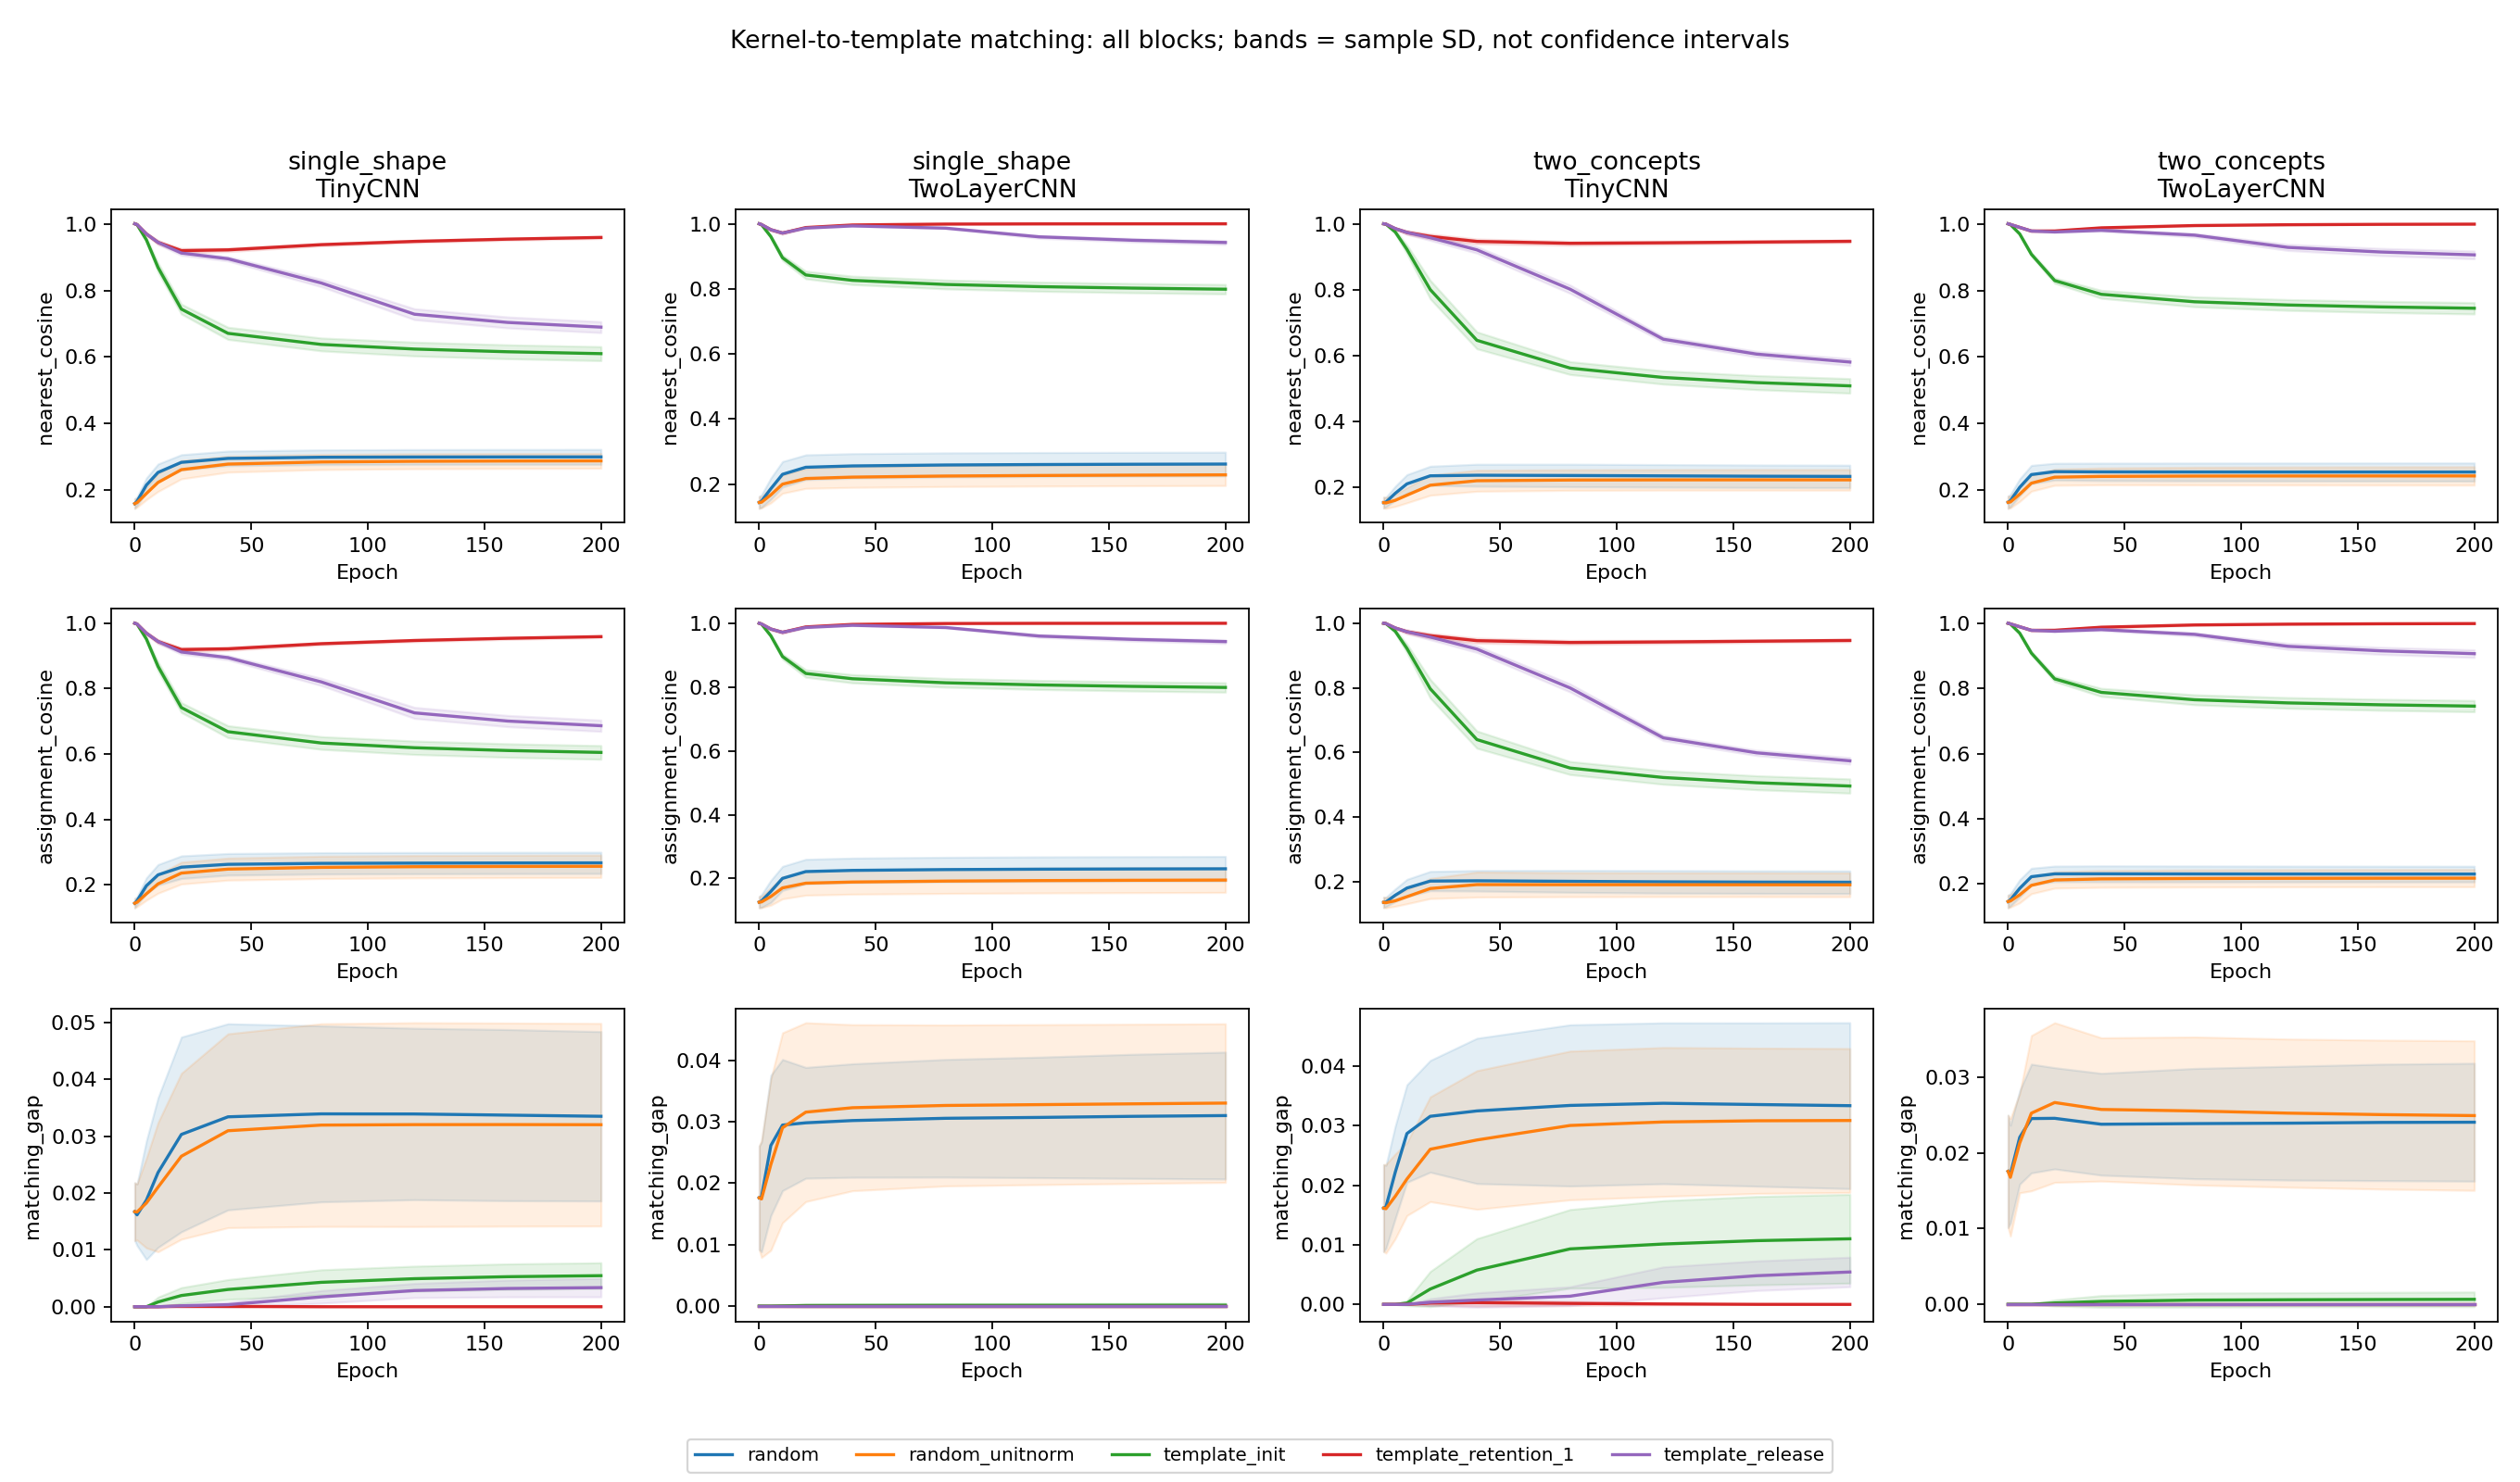
\includegraphics[width=\linewidth]{../analysis/kernel_similarity/results/matching_trajectories.png}
\caption{Nearest-template alignment, maximum-weight one-to-one alignment, and
their gap over all saved epochs. All five conditions and four settings are
shown. Bands are sample SD over ten blocks, not confidence intervals.}
\end{figure}
\begin{figure}[p]
\centering
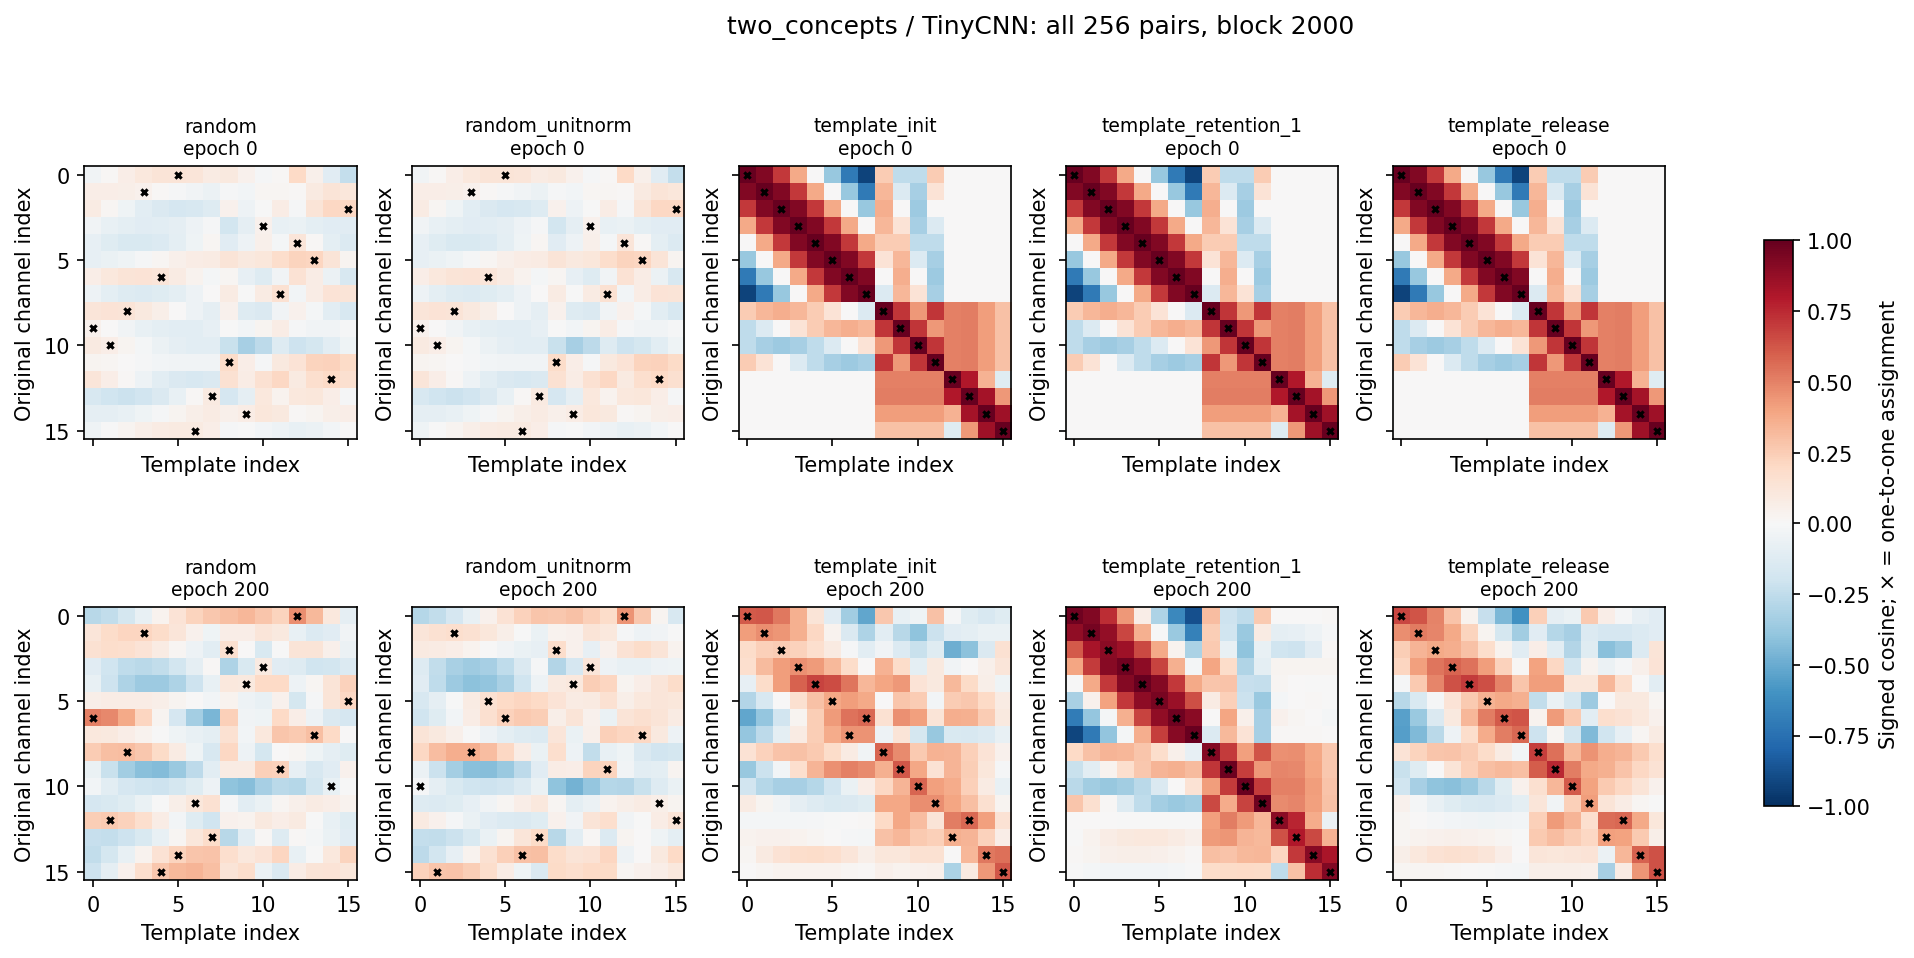
\includegraphics[width=\linewidth]{../analysis/kernel_similarity/results/matrices_two_concepts_TinyCNN.png}
\caption{All 256 signed kernel/template similarities for each condition at
initialization and epoch 200, two\_concepts/TinyCNN, fixed block 2000.
Rows retain original channel indices, columns retain template indices;
black crosses mark the optimal one-to-one assignment. Values range from
$-1$ to $1$. Matrices and galleries for all settings are retained in the
derived analysis artifacts.}
\end{figure}


\end{document}